\documentclass[11pt,twoside]{report} % Two side gjør det tosidig
\usepackage[utf8]{inputenc}
\usepackage{graphicx}
\graphicspath{{images/}}
% Konfigurerer page layout, default er US paper. Endrer på width også, og top/bottom margin.
\usepackage[a4paper,width=150mm,top=25mm,bottom=25mm,bindingoffset=2mm]{geometry}

\usepackage{setspace}
\linespread{1.25}

% for caption top tables
\usepackage{floatrow}
\floatsetup[table]{capposition=top}

% FancyHdr pakken gjør det mulig å legge til header og footer
\usepackage{fancyhdr}
\fancyhf{}
\pagestyle{fancy} % legger til default
% Endrer på header.
\fancyhead{}
\fancyhead[RO,LE]{\rightmark} %Ønsker thesis tittel på høyre side på oddetallssider, og venstre på partallsider.
\fancyhead[RE,LO]{\thepage}

\setlength{\headheight}{14pt}

%endrer på størrelse på skrift
\renewcommand{\headrulewidth}{0.4pt}
%\renewcommand{\footrulewidth}{0.4pt}

% bruk \pagestyle{empty} for å fjerne alt, og \pagestyle{plain} for å ha sidenummer på underkapitler (sections).
% Husk å bytte til fancy ved neste avsnitt eller der du vil ha fancy greier.

\usepackage[Glenn]{fncychap}

\usepackage{import}

% For enumerate

\usepackage{easylist}
\usepackage{paralist}

% for Bibtex
\usepackage{cite}

% For block quote
\usepackage{csquotes}

\usepackage{parskip}  % Separate paragraphs with a blank line
                      % rather than using indentation
\usepackage{url}
\usepackage{float} % for bildeplassering der du vil

\usepackage[colorlinks=true, a4paper=true, pdfstartview=FitV,
linkcolor=blue, citecolor=blue, urlcolor=blue]{hyperref}

% For new page
\usepackage{afterpage}
\newcommand\blankpage{%
	\null
	\thispagestyle{empty}%
	\addtocounter{page}{-1}%
	\newpage}


%%%%%%%%%%%%%%%%%%%%%%%%%%%%%% SETUP DOCUMENT %%%%%%%%%%%%%%%%%%%%%%%%%%%%%

\begin{document}
	\pagestyle{plain}
	% !TEX encoding = UTF-8 Unicode
%!TEX root = main.tex
% !TEX spellcheck = en-US

%This is the Titlepage
%%=========================================
\thispagestyle{empty}
%
\includegraphics[scale=1.1]{ntnu}
\mbox{}\\[6pc]

\begin{center}
\Huge{\textbf{Investigating Design Debt in Safety-Critical Systems: A Case Study}}\\[4pc]
\Large{Shahariar Kabir Bhuiyan}\\[1pc]


\noindent Master of Science in Computer Science
\linebreak
\noindent Submission Date: June 2016
\linebreak
\noindent Supervisor: Carl-Fredrik Sørensen
\linebreak
\linebreak
\noindent Department of Computer and Information Science\\
\noindent Norwegian University of Science and Technology
\end{center}

\vfill



	\afterpage{\blankpage}

	\setcounter{page}{0}
	\pagenumbering{roman}

	% !TEX encoding = UTF-8 Unicode
% !TEX root = ..\main.tex
% !TEX spellcheck = en-US
%%=========================================

%==========
% Abstract
%==========
%1. State the problem.
%2. Say why it's an interesting problem.
%3. Say what your solution achieves.
%4. Say what follows from your solution.

% Context, objective, method, results, conclusion
%\pagestyle{fancy}
%\fancyhf{}
%\renewcommand{\chaptermark}[1]{\markboth{\chaptername\ \thechapter.\ #1}{}}
%\renewcommand{\sectionmark}[1]{\markright{\thesection\ #1}}
%\renewcommand{\headrulewidth}{0.1ex}
%\renewcommand{\footrulewidth}{0.1ex}
%\fancyfoot{LE,RO}{\thepage}
%\fancypagestyle{plain}{\fancyhf{}\fancyloot[LE,RO]{\thepage}\reneewcommand{\headrulewidth}{0ex}}

\section*{\Huge Abstract}
\addcontentsline{toc}{chapter}{Abstract}
Software is contributing a substantial part of new functionality and innovations in safety-critical systems. These systems put a huge demand on software reliability, because a minor error can produce failure of a complete system. The evolution of software requires continuous development and maintenance. With size and complexity of safety-critical software growing as time goes, additional challenges arises. \textit{Technical debt} refers to the compromises that are made in software development and maintenance in order to meet a short-term business goal. \textit{Design debt} is an instance of technical debt. As software systems evolve, their design tend to decay over time, hence accumulating design debt. Consequently, software design becomes more difficult to maintain. Therefore, developers need to understand the reason for design debt accumulation so they can take proactive steps that may potentially reduce the debt in the future.

The main goal of this thesis is to empirically investigate design debt in safety-critical systems. The goal is reflected in our attempt to answer the following research questions:
\begin{itemize}
\item \textbf{RQ1:} How can design debt be identified?
\item \textbf{RQ2:} What kind of design debt can be found in embedded systems?
\item \textbf{RQ3:} What are the effects of design debt?
\item \textbf{RQ4:} How to pay design debt? 
\end{itemize}

A case study has been conducted in order to answer our research questions. The case study involves an analysis of a safety-critical system developed by Autronica Fire and Security AS. The system is written in C/C++. We used object-oriented metrics to identify classes that are most likely to pose problems for the system. Qualitative data were collected and analyzed using descriptive statistics. A set of thresholds for the metrics were derived to identify classes that have higher metric values than threshold values. In addition, automatic static analysis tools were applied in order to detect code smells. 

This work contributes mainly to the improvement in software metrics and software quality. The main contributions of this work:
\begin{easylist}[itemize]
& \textbf{C1:} Empirical knowledge about identification of design debt in safety-critical systems by object-oriented metric analysis and code smell detection.
&& \textbf{C1.1:} A set of threshold values for the measured object-oriented metrics
& \textbf{C2:} Empirical knowledge about the different types of design debt in safety-critical systems
& \textbf{C3:} Empirical knowledge about the effects of having design debt in safety-critical systems
%\item \textbf{C4} Empirical knowledge about refactoring possibilities of design debt
\end{easylist}
	\afterpage{\null\newpage}
	% !TEX encoding = UTF-8 Unicode
% !TEX root = ..\main.tex
% !TEX spellcheck = en-US
%%=========================================
\section*{\Huge Preface}
\addcontentsline{toc}{chapter}{Preface}
Here is the preface

	\afterpage{\null\newpage}
	\tableofcontents

	\clearpage
	\listoffigures

	\clearpage
	\setcounter{page}{0}
	\pagenumbering{arabic}
	\pagestyle{fancy}

	% !TEX encoding = UTF-8 Unicode
% !TEX root = ..\main.tex
% !TEX spellcheck = en-US

\chapter{Introduction}

This chapter provides an introduction to this masters thesis. We begin with outlining the motivation and context for the research. Then a brief description of the research questions is presented. Thesis outline is presented in the last section.


\section{Motivation and Background}
The field of embedded systems is growing rapidly based on the evolution in electronics and widespread use of sensors and actuators. From consumer electronics, automobiles, to satellites, embedded systems represent one of the largest segments of the software industry. Embedded systems are forecasted to grow exponentially in the next 10 years\cite{graaf2003embedded}. Software plays a central role in the development of embedded systems. Embedded software is the primary driving force for implementing different funcitonalities of todays embedded systems. The sotware is specialized for one particular hardware, and may therefore introduce hardware specific run-time constraints. In this context, the quality of software systems becomes crucial. 

According to Gartner\cite{gartner2010}, the cost of dealing with technical debt threatens to grow to \$1 trillion globally by 2015. That is the double of the amount of technical debt in 2010. 

\section{Research Context}


\section{Research Questions}


\section{Thesis Structure}
The thesis is structured into several chapters with sections and subsections. The outline of the thesis is as follows:
\begin{itemize}
	\item{\textbf{Chapter 1}}: Introduction contains a brief and general introduction to the study and the motivation behind it.
	\item{\textbf{Chapter 2}}: State-of-the-Art looks at important aspects of the research question.
	\item{\textbf{Chapter 3}}: Research Method describes how the literature review was carried out throughout the research, as well as a description of the case study to be performed.
	\item{\textbf{Chapter 4}}: Results presents the results from the case study, and takes a closer look at the findings from the case study.
	\item{\textbf{Chapter 5}}: Discussion contains a summarized look at the findings from the case study, and connects it with the literature review and to the research questions. An evaluation of the research is also given in this chapter.
	\item{\textbf{Chapter 6}}: Conclusion concludes the research by providing a summary of the most important points of the results and discussion chapter. Additionally, in outlines possible routes to take in the research field.
\end{itemize}


	% !TEX root = ..\main.tex
\chapter{State-of-the-Art}
This chapter presentes topics which are relevant to this project. Section 2.1 looks into technical debt with its definitions, types etc. Section 2.2 looks into embedded systems and some of the challenges with it. Section 2.3 presents 


\section{Technical Debt}
The concept of technical debt was first introduced by Ward Cunningham in 1992 to communicate the problem with non-technical stakeholders\cite{p29-cunningham}. The concept was used to describe the system design trade-offs that are made everyday. To deliver business functionality as quickly as possible, \textit{'quick and dirty'} decisions leading to technical debt had to be made, which affect future development activities. Cunningham further describes technical debt as \textit{"shipping first time code is like going into debt. A little debt speeds development as long as it is paid back promptly with a rewrite"}. As time goes, technical debt accumulates interest leading to increased costs of a software system\cite{p31-guo,p35-klinger}. However, not all debts are necessarily bad. A small portion of debt might help developers speed up the development process in the short-term\cite{p31-guo}. 


%% The costs of technical debt
\begin{figure}[ht!]
	\centering
	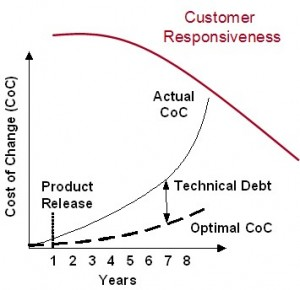
\includegraphics[width=0.8\textwidth]{images/techdebtCurve.jpg}
	\caption{The Technical Debt Curve\cite{jim-highsmith}}
	\label{fig:techDebtCurve}
\end{figure}

Figure \ref{fig:techDebtCurve} illustrates what happens as technical debt grows over time within a software product. Once we are on the far right of the curve, all choices are hard. The software controls us more than we control it.

%%%

\subsection{Definitions of Technical Debt}
McConnell describes TD as: \textit{a design or construction approach that is expedient in the short term but that creates a technical context in which the same work will cost more to do later than it would cost to do now (including the increased cost over time)}. He further splits the term into two categories based on how they are incurred, intentionally or unintentionally\cite{url-mcconnell}. The unintentional category includes debt that comes from doing a poor job. For example, uninntentional debt might be when a junior software developer writes bad code due to lack of knowledge and experience. Intentional debt occurs when an organization makes a decision to optimize for the present rather than the future. An example is when the project release must be done on time, or else there will not be a next release. This leads to bad decisions, like taking a shortcut to solve a problem, and then reconcile the problem after shipment

Fowlers presents a more formal explanation of how technical debt can occur\cite{url-fowler}. He categories technical debt into a quadrant with two dimensions, which he calls the \textit{"Technical Debt Quadrant"}. As seen in the Figure \ref{fig:techDebtQuad}, the debt is grouped into four categories: 

\begin{figure}[ht!]
	\centering
	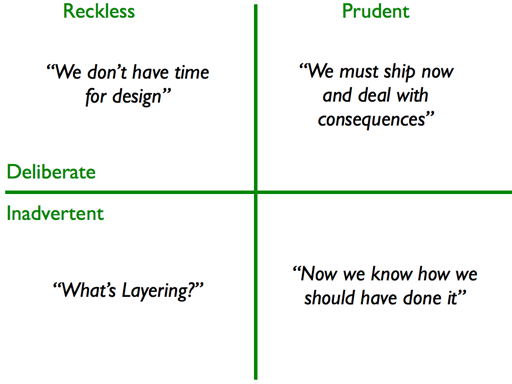
\includegraphics[width=0.8\textwidth]{images/techDebtQuadrant.png}
	\caption{Technical Debt Quadrant}
	\label{fig:techDebtQuad}
\end{figure}

\begin{itemize}
	\item \textbf{Reckless/Deliberate debt}: The team feels time pressure, and takes shortcuts intentionally without any thoughts on how to address the consequences in the future.
	\item \textbf{Reckless/Inadvertent debt}: Best practices when it comes to code and design is ignored, and a big mess in the codebase is made.
	\item \textbf{Prudent/Deliberate debt}: : The value of taking shortcuts is worth the cost of incurring debt in order to meet a deadline. The team is aware of the consequences, and has a plan in place to address them in the future. 
	\item \textbf{Prudent/Inadvertent debt}: Software development process is as much learning as it is coding. The team can deliver a valuable software with clean code, but in the end they might realize that the design could have been better.
\end{itemize}

Krutchen divides technical debt into two categories\cite{krutchen}. Visible debt that is visible for everyone. It containts elements such as new functionality to add and defects to fix. Invisible is the other category, debt that is only visible to software developers. Figure \ref{fig:techDebtLandscape} shows a map of the "technical debt landscape" which helps us to distinguish visible and invisible elements. On the left side of Figure \ref{fig:techDebtLandscape}, TD mostly affects the evolvability of the software system, while on the right it mainly affects maintainability.

\begin{figure}[ht!]
	\centering
	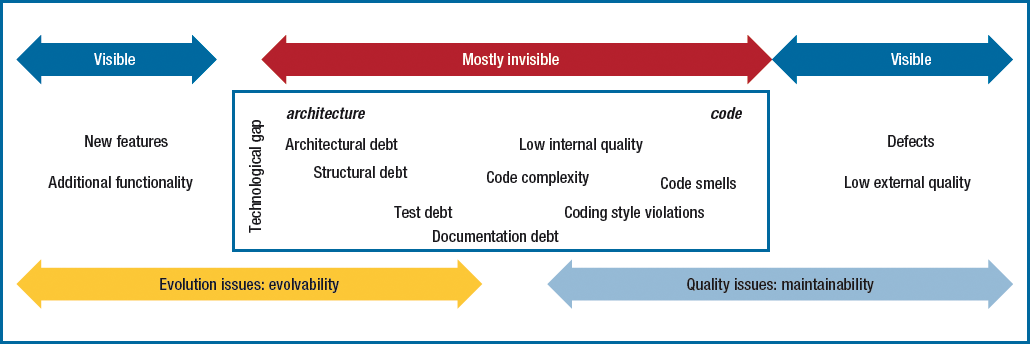
\includegraphics[width=1.0\textwidth]{images/techDebtLandscape.png}
	\caption{Technical Debt Landscaape}
	\label{fig:techDebtLandscape}
\end{figure}

\subsection{Comparison with financial debt}
Technical debt has many similarities to financial debt\cite{p50-allman,Zazworka:2011:PDD:1985362.1985372}:
\begin{itemize}
	\item You take a loan that has to be repaid later
	\item You usually repay the loan with interest
	\item If you can not pay back, a very high cost will follow. For example, you can loose your house or car.
\end{itemize}

Like financial debt, technical debt accrues interest over time which comes in the form of extra effort that has to be dedicated in future development because of bad choices\cite{p31-guo,p35-klinger}. Stakeholders can choose to continue paying the interest, or you can pay down the debt by refactoring the code or system into something better which reduces interest payments in the future\cite{url-fowler}. If the debt is not repaid, development might slow down, e.g, due to poor maintainability of the code. This can lead to software project failure and you might go bankrupt\cite{p50-allman}. There are some differences between financial and technical debt as well. The debt has to be repaid eventually, but not on any fixed schedule\cite{p50-allman}. This means that some debts may never have to be paid back, which depends on the interest and the cost of paying back the debt\cite{foser076-brown}. Example on interests can be be lower pace of development, low competitiveness, security flaws on the system, loss of developers and their expertise, poor internal collaboration environment, dissatisfied customers, and loss of market share\cite{p50-allman}.


\subsection{Causes and effects of technical debt}
Multiple studies have tried to analyze the reason for companies to incur technical debt.

%While financial debt occus from deliberate actions of taking a loan, technical debt may be caused by several factors. Antares categories these factors into four groups:
%\begin{itemize}
%	\item Work processes: Software development methology, can some tasks be automized (with a deploy script), is tests written after bug fixing, do you map and document shortcuts you take, is there any plans for techincal debt management later, is it important to implement new functionality or to make sure that the existing ones work propertly?
%	\item People (knowledge and capacity): Do you need some individuals to finish a task, Do you have the right people for the job, is enough training given to new people, what happens if you need someone who's on vacation/change project/is sick or something. You should keep this in mind and make a plan on how knowledge is transferred. Techcnical debt can be the reason for poor motivation and productivity which causes you to work poorly. 
%	\item Technology: Is solutions hard to integrate with other solutions, is all the systems out there compatible with newer technology, is there any outdated or duplicated code in the system, is all the systems secure, is the solutions old, or user friendly, is there some code which is hard to maintencance. 
%	\item Collaboration in the organization: Commuinication between developers and requirement people. You often get a list with requirements, is the list understandable? Do we work with a backlog with tasks that should have been solved long time ago, but not which is not "actual" now?
%\end{itemize}
%Developers might not care about the product because they don't feel that they "own" what's being made. They get told what do to, but not more than that. Can't make requirements.


%Operating technical debt might be to maintenance and manage existing code rather than implementing new functionality. It is important to keep track of the technical debt, and incur interest payments, before it makes troubles for you. Do do that, you could for example set up a plan for repayment which tells you something about how the debt shall be repayed. Scrum can be used to do this for example, where you split the repayment plan to smaller parts where you estimate and prioritize tasks. It is important to remember that taking too much loan might cause problems. As mentioned ealier, technical debt can be seen as taking a financial loan according to Cunningham. The loan has to be repaid with interests. Technical debt uses time and effort as repayment. It is acceptable to take a loan, but it should be controlled. Do not take loan than what you are able to handle. Think with your head.

%Main developers behind a software project aren't the one who usually maintain the code. Companies often has policies where they transfer a project to new developers after the development phase is over. The reasons could be to save money, or that the new developers might work more. These maintenance people often haas to repay the debt. The main developers gets awarded for their implementation speed rather than thinking on maintanence and evolution. They can often be placed on new projects before the debt has to be paid back, making them unavaiable for a period. Too few systems also has TODO or FIXME comments in their source code.

Klinger et al.\cite{p35-klinger} carried out an industrial case study at IBM where four technical architects with different backgrounds were interviewed. The goal was to examine how the decisions to incur debt were taken, and the extent to which the debt provided leverage\cite{p35-klinger}. The study revealed that the company failed to assess the impact of intentionally incurring debt on projects. Decisions regarding technical debt were rarely quantified. The study also revealed big organizational gaps among the business, operational, and technical stakeholders, which incurred debt. When the project team felt pressure from the stakeholders, technical debt decisions were made without quantifications of possible impacts.

Lim et al.\cite{lim-taksande} show that technical debt is not always the result of poor developer disciplines, or sloppy programming. It can also include intentionals decisisions to trade off competing concerns during business pressure. They also found out that technical debt can be used in short term to capture market share and to collect customers feedback early. In the long term, techical debt tended to be negative. These tradeoffs included increased complexity, reduced performance, low maintainability, and fragile code. This led to bad customer satisfaction and extra working hours. In come cases, the short term benefits of technical debt outweighted the future costs.

Guo et al.\cite{guo2011tracking} studied the effects of technical debt by tracking a single delayed maintenance task in a real software project throughout its lifecycle, and simulated how managing technical debt can impact the project result. The results showed that delaying the maintenance task would have almost tripled the costs, if it had been done later.

Siebra et al.\cite{p247-siebra} carried out an industrial case study where they analyzed documents, emails code files, and had interviews with developers and project managers. This case lasted for six years. This study revealed that technical debt were mainly taken by strategic decisions. They also found out that using a unique specialist could lead the development team to solutions that the specialist wanted and believe were correct, leading the team to incur debt. The study also identified that technical debt can both increase and decrease the amount of working hours.

Zazworka et al.\cite{zazworka2011investigating} studied the effects of god classes and technical debt on software quality. God classes are examples on bad coding, and therefore includes a possibility for refactoring\cite{Zazworka:2011:PDD:1985362.1985372}. The results indicated that god classes require more maintenance effort including bug fixing and changes to software that are considered as a cost to software project. In other words, if developers desire higher software quality, then technical debt needs to be addressed closely in the development process.

Buschmann\cite{buschmann2011pay} explained three different stories of technical debt effects. In the first case, technical debt in one platform started to grow so large that development, testing, and maintenance costs started to increase dramatically, and the components were hardly usuable. In the second case, developers started to use shortcuts to increase the development speed. This resulted in significant performance issues because an improper software modularization reflected organizational structures instead of the system domains. It ended up turning in to economic consequences. In the third case, an existing software product experienced increased maintainenance cost due to architecture erosion. However, management analyzed that reengineering the whole software would cost more than doing nothing. This resulted in a situation where the management decided not to do anything to technical debt, because it was cheaper from a business point-of-view.

Codabux et al.\cite{p8-codabux} carried out an industrial case study where the topic was agile development focusing on techincal debt. They observed and interviewed developers to understand how technical debt is characterized, addressed, prioritized, and how decisions led to technical debt. They defined two subcategories of technical debt; infrastructure and automation debt. 

These studies indicates that the causes and effects of technical debt are not always caused by technical reasons. Technical debt can be the result of intentional decisions by the stakeholders. Incurring technical debt may have short-term positive effects such as time-to-market benefit. The tradeoffs are economic consequences, and quality issues in the long run if debt is not paid back. The allowance of technical debt can facilitate product development for a period, but decreases the product maintainability in the long term. However, there are some times where short-term benefits overweight long-term costs. 

These studies points out that several types of technical debt are related to software lifecycle phases. The effects of taking shortcuts can happen in several stages of software lifecycle. Table \ref{tab:subcategories} lists the types of technical debt that has been identified in these studies.

\begin{table}
	\centering
	\begin{tabular}{ | p{5cm} | p{8cm} |}
	\hline
	\textbf{Subcategory} & \textbf{Definition} \\ \hline
	Architectural debt\cite{li2015systematic,p8-codabux,foser076-brown} & Architectural decisions that make compromises in some of the quality attributes, such as modifiability. \\ \hline
	Code debt\cite{li2015systematic,foser076-brown,tom2013exploration} & Poorly written code that violates best coding practices and guidelines, such as code duplication. \\ \hline
	Defect debt\cite{li2015systematic,tom2013exploration} & Defect, failures, or bugs in the software. \\ \hline
	Design debt\cite{li2015systematic,Zazworka:2011:PDD:1985362.1985372,foser076-brown} & Technical shortcuts that are taken in design.\\ \hline
	Documentation debt\cite{li2015systematic,foser076-brown,Zazworka:2013:CSE:2460999.2461005} & Refers to insufficient, incomplete, or outdated documentation in any aspect of software development.\\ \hline
	Infrastructure debt\cite{li2015systematic,tom2013exploration,p8-codabux} & Refers to sub-optimal configuration of development-related processes, technologies, and supporting tools. An example is lack of continious integration.\\ \hline
	Requirements debt\cite{li2015systematic,Zazworka:2013:CSE:2460999.2461005} & Refers to the requirements that are not fully implemented, or the distance between actual requirements and implemented requirements.\\ \hline
	Test debt\cite{li2015systematic,Zazworka:2013:CSE:2460999.2461005,foser076-brown} & Refers to shortcuts taken in testing. An example is lack of unit tests, and integration tests.\\
	\hline
	\end{tabular}
	\caption{Types of technical debt} \label{tab:subcategories}
\end{table}

\subsection{Current strategies and practices for managing technical debt}
Managing technical debt compromises the actions of identifying the debt and making decisions about which debt should be repaid\cite{foser076-brown,krutchen,url-mcconnell}. This section examines some proposed methods

Brown et al.\cite{foser076-brown} proposes open research questions to understand the need to manage technical debt. The questions includes refactoring opportunities, architectural issues, identifying dominant sources of technical debt, and identifying issues that arise when measuring technical debt.

%Lim.et al - 4 strategies
Lim et al.\cite{lim-taksande} found four strategies for managing technical debt. The first strategy is to do nothing because the technical debt might never be visible to the customer. The second strategy is to use a risk management approach to evaluate and prioritize technical debt's cost and value by allocating five to ten percent of each release cycle to address technical debt. The third strategy is to include the customers and non-technical stakeholders to technical debt decisions. The last strategy is to track technical debt using tools like a Wiki, or a backlog.

%Codabux
Codabux et al.\cite{p8-codabux} suggests best practices such as refactoring, repackaging, reengineering, and developing unit tests to manage technical debt. They also suggest having dedicated teams with the purpose of reducing technical debt, while the product development team devote 20\% of their effort toward technical debt reduction.
	
%Portifolio management (guo, zazworka (priorizing design debt investment opportunities))
Guo et al.\cite{p31-guo} suggest the use of portfolio management for technical debt management. This approach collects technical debt to a \textit{"Technical Debt List"} (TDL) that is being used to pay the technical debt back based on its cost and value. Three activities support the TDL. The first activity is Technical Debt Identification. This activity use several tools to identify technical debt items which are then automatically placed in the TDL. The second activity is Technical Debt Estimation. Each item in the list is assigned the estimates for the debt principal, and the interest. The third activity, Decision Making, is used to determine which debts should be addressed first, and when they should be addressed.

%Quantifying technical debt - Nugraho
Nugraho et al.\cite{p1-nugraho} proposes an approach to quantify technical debt and its interest by using a software quality assessment method. This method rates the technical quality of a system in terms of the quality characteristics of ISO9126. 

%Krutchen (define tech debt in your backlog)
Krutchen\cite{krutchen} suggests listing debt-related tasks in a common backlog during release and iteration planning. Figure \ref{fig:fourColorBacklog} illustrates how these elements can be organized in a backlog. Krutchen further mentions that project backlogs often contain the green elements. The rest are seen rarely, especially the black elements, they are nowhere to be found.


\begin{figure}[ht!]
	\centering
	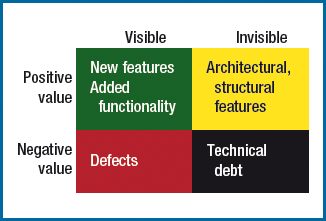
\includegraphics[width=0.8\textwidth]{images/fourColorBacklog.png}
	\caption{The colors reconcile four types of possible improvements.}
	\label{fig:fourColorBacklog}
\end{figure}

SonarQube is an open source application for quality management. It manages results of various code analysis tools, and is used to analyze and measure a projects technical quality. The technical debt is computed based on the SQALE (Software Quality Assessment based on Lifecycle Expectations) methodology. SQALE is a method for assessing technical debt in a project. It is based on tools that analyze the source code of the project, looking at different types of errors such as mismatched indentation, and different naming conventions. Each error is assigned a score based on how much work it would take to fix that error. The analysis gives a total sum of technical debt for the entire project.



%\subsection{Organizational debt}
%While technical debt is known problem, there's one more type of debt which can be accrued on a compandy-wide level. This type of debt is called organizational debt. Organizational debt is all about people and culture compromises made to \textit{'just get it done'} in early stages of a startup, preventing a company from running smoothly\cite{steve-blank}. When things should be going great, organizational debt can turn a growing company to a nightmare. Growing companies needs to know how to recognize and refactor organizational debt. 

%Some of the causes behind organizational debt might be:

%\begin{itemize}
%	\item Training the new hires, both culture and specific tasks
%	\item Retain existing hire by doing something for them. Many doesn't get promoted. New hire might get a better posistion than existing hire who has been there from the start.
%\end{itemize}

%Sometimes, the employees gets awarded by good building, new furnitures, and compensation for executive staff. However, that isn't enough. Think about existing employees who's been there from the start. You might end up loosing qualified people who's spent years building up the company, but not compensated for it. Top-down approach is focused too much. Think about the bottom employees.They have the inistituinal knowledge and hard-earned skills.

%When new people got hired, the ones who could train them about the company culture and how to do their specific tasks is the old employees who's being underpaid. They will look for another job. No one would be able to train the new people then. Giving compensation in form of stock vesting, insurance benefits, movie nights etc isnt enough as everyone gets it. Do something for the employees who's been there for a long time.

%Refarocting might be important in order to reduce the organizational debt. Write plan for managing new wave of hires before hiring them. Sometimes, you'll also need to think about what you will have to do if you're about to loose a key employee. Is it worth to replace employees who hold critical knowledge? Put together an expence budget using the current employee salaries. See who's important. Identify the one they wanted to keep and upgrade them. Some employees might not be that important as welll as they might be a performance problem for the whole organization. Need to look at the company culture as well, does it take into account of the new size and stage of the organization? What have the company achieved, what are the key elements that have made it great so farm, are they same of different. Think about the customer too. Does we talk to the customer, or does the customer talk to us. Also, keep in mind that an adivosory board of other CEOS who've been through the early stages might be good. Failure to refactor might kill a growing company\cite{steve-blank}.

%Some examples on organizational debt:
%\begin{itemize}
%	\item Different departments solving the same problems might use differnet methologies and tools. Difficult to see similarities in order to address company-wide issues.
%	\item Creation of processes and implement solutions which seems great at first, but didnt address the root casue of the issue and ending up creating more problems.
%	\item Time constraints, solving a problem in less-than-ideal manner this time. This manner is repeated because no one remember that the first time was intended to be one-off situation.
%\end{itemize}

%%%%%%%%%%%%%%%%%%%%%%%%%%%%%%%%%%%%%%%%%%%%%%%%%%%%%%%%%%%%%%%%%%%%%%%%%%%%%%%%%%%%%%

			% SOFTWARE LIFECYCLE

%%%%%%%%%%%%%%%%%%%%%%%%%%%%%%%%%%%%%%%%%%%%%%%%%%%%%%%%%%%%%%%%%%%%%%%%%%%%%%%%%%%%%%

\section{Software Lifecycle}
A software lifecycle is the phases a software product goes through between its convenient and when its no longer available for use\cite{159431}. There are five general groups of related activities in the software lifecycle according to IEEE Standard for Developing Software Life Cycle Processes\cite{159431}. 

\begin{enumerate}
	\item The first group is project management. Every software lifecycle starts with the project initiation. Project planning, and project monitoring and control are two other, necessary activities withing this group for each project iteration. 
	\item The second group is of pre-development. This group consists of activities that needs to be performed before the software development phase. Concept exploration is a good example of such activity. 
	\item The third group is the development itself. It includes the activities that must be performed during the development.
	\item The fourth group is of post-development. It includes activities to be performed after development to enchance the software project. The retirement activity involves removal of the existing system from its active support by ceasing its operation or support, or replacing it with a new system or an upgraded version of the exisiting system. 
	\item The final group is called integral. This group consists of activities that are necessary to ensure successful completion of a project. These activities is seen as support activities rather than activities that are directly oriented to the development effort.
\end{enumerate}

\subsection{Software Development Life Cycle and Methodologies} % (fold)
A software development process or a software development lifecycle is defined as the process by which user needs are translated into a software product\cite{radatz1990ieee}. The process involves translating user needs into requirements, transforming requirements into design, implementing design into code, testing the code, and sometimes, installing and checking out the software for operational use.

A software development methodology is defined as a framework to structure, plan, and control the software development process. Many software development methodologies exists, and the basic lifecycle activities are included in all lifecycle models, often in different orders. The difference is in terms of time to release, risk management, and quality. The models can be of different types, but they are usually defined as traditional and agile software development methodologies.

\subsubsection{Traditional Software Development}
Traditional software development methodologies are based on a sequential series of steps. It usually starts with elicitation and documentation of a complete set of requirements, followed by architecture and high level design, development, testing, and deployment. The most well-known of these traditional software development methodologies is the Waterfall method, the oldest software development process model. The Waterfall Model divides the software development lifecycle into five distinct and linear stages\cite{Vliet:2008:SEP:1481475}; requirements engineering, design, implementation, testing, and maintenance. There are many risks associated with the use of Waterfall model\cite{hijazi2012review}:
\begin{itemize}
	\item \textbf{Continuous requirements change}: Requirements are specified at the beginning of the software development process, and the remaining software development activities have to follow the initial requirements. This kind of model is not appropiate to use for software where technology and business requirements always change. 
	\item \textbf{No overlapping between stages}: Each stage in the Waterfall model needs to be completed entirely before proceeding into the next phase.
	\item \textbf{Poor quality assurance}: Lack of quality assurance during the differnet phases is another source of risk. Testing the system is the last stage in the development prorcess. Thus, all problems, bugs, and risk are discovered too late.
	\item \textbf{Relatively long stages}: Long stages in the development process makes it difficult to estimate time and cost. Additionally, there is no working product until late in the development process. 
\end{itemize}

Using sequential design processes such as Waterfall model in software development processes to build complex, intensive systems is often a failure\cite{p50-allman}. According to the Standish Group, CHAOS Report of 2015 reveals that 29\% of all projects using Waterfall method tends to fail, with no useful software deployed. 

%This is why agile methods was made, where change and feedback is important. One of the benefits is the ability to quickly release new functionality. However, one of the problems with agile methods is that developers often wants to focus on implementing new fucntionality, which results in poor focus on design, code quality, testing, which again leads to technical debt.  

\subsubsection{Agile Methods}
To address the challenges posed by traditional methods, agile methods were developed as a set of lightweight methods\cite{hijazi2012review}. Agile methods try to deal with collaboration in a way that promotes adaptive planning, early delivery, and continuous improvement, making the development phase faster and more flexible regarding changes\cite{abrahamsson2002agile}. Agile Manifesto describes four values that defines agile software development\cite{agilemanifesto}: 
\begin{itemize}
	\item Individuals and interactions over processes and tools
	\item Working software over comprehensive documentation
	\item Customer collaboration over contract negotiation
	\item Responding to change over following a plan
\end{itemize}

\textbf{Scrum} is one of the most popular agile software development methodologies. It is an iterative and incremental software development model. An advantage with iterative procedures is that parts of a system is developed early on, and can be tested before implementation of other parts. This reduces the risk of having long stages. The idea with Scrum is to divide the development into short periods, called sprints. Unlike the approach in the Waterfall model, the team can estimate how long it will take to implement tasks which can be accomplished during each sprint. To implement the requirements step by step, a product backlog is kept containing the features that have yet to be implemented. The product backlog is not static as it changes to the needs of the project, with new features being added, and obsolete ones being removed. Sprint backlog is items from the backlog that a team works on during a sprint.

\textbf{Lean Development} adapts the concepts and principles of Toyota Product Development System, to the practice of developing software\cite{Poppendieck:2007:LSD:1248821.1248986}. It is seen as a key component in building a change tolerant business\cite{cawley2010lean}. The seven lean principles that is applied to software development can be summarized as \textit{eliminate waste, build quality in, create knowledge, defer commitment, deliver fast, respect people, and optimize the whole}\cite{Pressman:2009:SEP:1593949,Poppendieck:2007:LSD:1248821.1248986}. These principles has many similarities with the Agile Manifesto.

Moreover, there are many risks associated with agile methodologies\cite{hijazi2012review}:
\begin{itemize}
	\item \textbf{Very large software system}: Developing large, complex software systems results in large increments. This increase the time span between increments, and thus require a higher cost to deal with changes and bugs if discovered.
	\item \textbf{Large development team}: Having large teams results in difficulities in managing communication between team members.
	\item \textbf{High reliance on human factor}: Agile methodologies relies on the development team, and their abilities to communicate with the customers.
	\item \textbf{Inappropriate customer representative}: This factor can influence the development process and the team members.
	\item \textbf{Distributed development environment}: Agile methodologies requires close interaction between the development team. Having a distributed development environment might challenge the communication between team members due to different time zones.
	\item \textbf{Scope creep}: With minimal planning conducted, developers can be easily distracted from the project main objectives.
\end{itemize}


\begin{figure}
	\centering
	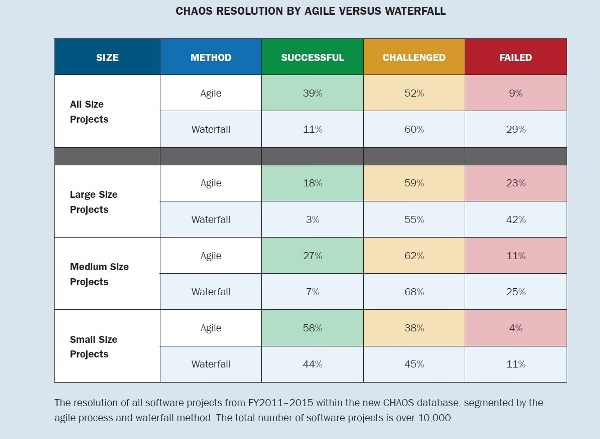
\includegraphics[width=0.8\textwidth]{images/Agile-Waterfall-Success-Failure-Rates.jpg}
	\caption{Agile implementation success rate by The Standish Group (SITER)}
	\label{fig:agileWaterfallSuccessFailureRates}
\end{figure}


%%%%%%%%%%%%%%%%%%%%%%%%%%%%%%%%%%%%%%%%%%%%%%%%%%%%%%%%%%%%%%%%%%%%%%%%%%%%%%%%%%%%%%

			% SOFTWARE ARCHITECTURE

%%%%%%%%%%%%%%%%%%%%%%%%%%%%%%%%%%%%%%%%%%%%%%%%%%%%%%%%%%%%%%%%%%%%%%%%%%%%%%%%%%%%%%
\section{Software Architecture}
Bass, Klements and Kazman\cite{Bass:2012:SAP:2392670} defines software architecture as following: 

\begin{displayquote}
The software architecture of a system is the set of structures needed to reason about the system, which compromise software elements, relations among them, and properties of both.
\end{displayquote}

The architecture of a software is one of the most important artifacts within the systems life cycle\cite{Bass:2012:SAP:2392670,knodel2006static}. Architectural design decisions that are made during the design phase, affect the systems ability to accept changes and to adapt to changing market requirements in the future. As the design decisions are made early, it will directly affect the evolution and maintenance phase\cite{Pressman:2009:SEP:1593949}, activities that consumes a big part of the systems lifespan\cite{Vliet:2008:SEP:1481475}. The problem of software architecture has long been a concern for those building and evolving large software systems\cite{perry1997state}.

Software architecture can be seen from two standpoints; prescriptive and descriptive architecture. The prescriptive architecture of a system captures the design decisions made prior to the construction. This is normally called as-conceived software architecture. Descriptive architecture describes how the system has actually been build, called for as-implemented software architecture. 

As the system evolves, it is ideal that the prescriptive architecture is modified first. In practice, the system - the descriptive architecture - is often directly modified. This can be due to developers sloppiness, short deadlines, or lack of documented prescriptive architecture. These principles introduces two new concepts; architectural drift and architectural erosion\cite{Bass:2012:SAP:2392670}. Architectural drift occurs when the documents are updated according to the implementation. The software architecture ends up as an architecture without vision and direction. Architectural erosion occurs when the implementation drifts away from the planned architecture. 

Long-term responsiveness of a system can be achieved by providing a solution of a system that would achieve certain quality attributes. The achievement of such quality attributes is based on the software architecure. 


%%%%%%%%%%%%%%%%%%%%%%%%%%%%%%%%%%%%%%%%%%%%%%%%%%%%%%%%%%%%%%%%%%%%%%%%%%%%%%%%%%%%%%

		% SOFTWARE MAINTENANCE AND EVOLUTION

%%%%%%%%%%%%%%%%%%%%%%%%%%%%%%%%%%%%%%%%%%%%%%%%%%%%%%%%%%%%%%%%%%%%%%%%%%%%%%%%%%%%%%
\section{Software Evolution}
Increasingly, more and more software developers are employed to maintain and evolve existing systems instead of developing new systems from scratch\cite{Sommerville:2011:SE}. Software evolution is a process that usually takes place when the initial development of a software project is done and was successful\cite{Bennett:2000:SME:336512.336534}. The goal of software evolution is to incorporate new user requirements in the application and adapt it to the existing application. Software evolution is important because it takes up to 85-90\% of organizational software costs\cite{Sommerville:2011:SE}. It is also important because technology tend to change rapidly, and not following these trend means loosing business oppertunities.

Rajlich and Bennet\cite{Bennett:2000:SME:336512.336534} proposed a view of the software lifespan, as shown in Figure \ref{fig:lifespan-1}. This view divides the software lifespan into five stages with initial development as the first stage. The key contribution is to seperate the maintenance phase into an evolution stage, followed by a service stage, and at last the phase-out stage.
\begin{description}
	\item[Initial development] produces the first version of the software from scratch.
	\item[Evolution] is the phase where significant changes to the software may be made. This could be addition of new features, correct previous mistakes, or adjust the software to new business requirements or technologies. Each change introduces a new feature or some other new property into the software.
	\item[Servicing] is the stage where relatively small, essential changes are allowed. The company considers how the software can be replaced. Legacy software is a term to describe software in this stage.
	\item[Phase-out] is the phase where software may still be used, but no further changes are being implemented. Users must work around any problems that they discover, or replace the software with something else.
	\item[Close-down] is when the managers or customers completely withdraw the system from production.
\end{description} 

\begin{figure}[ht!]
	\centering
	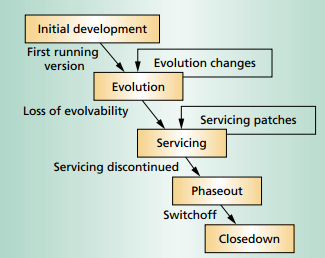
\includegraphics[width=0.8\textwidth]{images/lifespan-1.png}
	\caption{Software evolution process}
	\label{fig:lifespan-1}
\end{figure}

A variation of this process is the versioned stage model, as shown in Figure \ref{fig:lifespan-2}. When a software version is completed and released to the customer, the evolution continues with the company eventually releasing another version and only servicing the previous version. 

\begin{figure}[ht!]
	\centering
	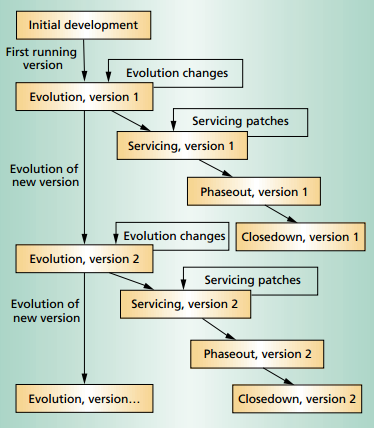
\includegraphics[width=0.8\textwidth]{images/lifespan-2.png}
	\caption{Software lifespan}
	\label{fig:lifespan-2}
\end{figure}

\subsection{Evolution Processes}
Software evolution usually starts with change proposals, which may be new requirements, existing requirements that have not been implemented, or bug reports from stakeholders. The process of implementing a change goes through these stages\cite{Sommerville:2011:SE} as shown in Figure \ref{fig:seProcess}.

The process starts with a set of proposed change requests. The cost and impact of the change is analyzed to decide whether to accept or deny the proposed changes. If the proposed changes are accepted, a new release of the system is planned. During release planning, all proposed changes such as fault repair, adaptation, and new functionality, are considered, to decide which changes to implement in the next version of the system. The changes are implemented and validated, and a new version of the system is released. The process ends with a new iteration with a set of proposed change requests for the next release. 

Sometimes, the need ofurgent changes may appear, such as a serious system fault that must be repaired to allow normal operation. In these cases, the usual process will not be beneficial as it takes time. An emergency fix is usually made to solve the problem. A developer choose a quick and workable solution rather than the best solution. The trade-off is that the the requirements, the software design, and the code become inconsistent. As a system changes over time, it will have impact on the systems internal structure and complexity. Software evolution might cause poor software quality and erosion of software architecture over time\cite{Bass:2012:SAP:2392670}.

\begin{figure}[h!]
	\centering
	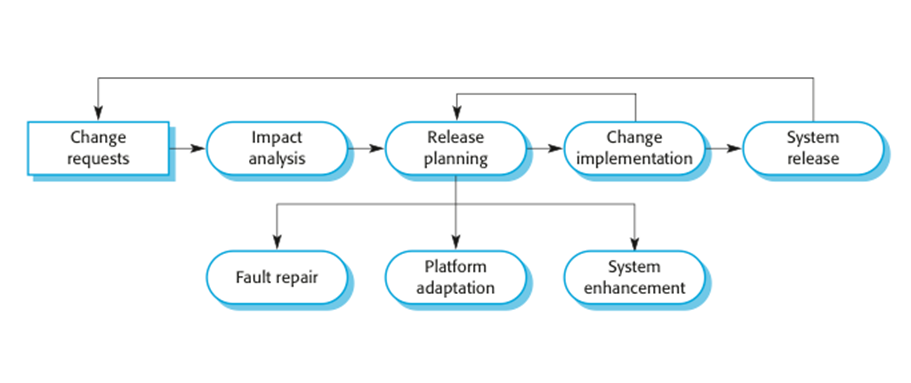
\includegraphics[width=0.8\textwidth]{images/SEprocess.png}
	\caption{Software evolution process}
	\label{fig:seProcess}
\end{figure}


\subsection{Software Maintenance}
IEEE 1219 defines software maintenance as follows\cite{720567}:
\begin{displayquote}
Modification of a software after delivery to correct faults, to improve performance or other attributes, or to adapt the product to a modified environment.
\end{displayquote} 
Maintenance can be classified into four types\cite{Bennett:2000:SME:336512.336534,720567}.

\begin{itemize}
	\item Adaptive: Modification of a software product performed after delivery to keep a computer program usable in a changed or changing environment.
	\item Perfective: Modification of a software product after delivery to improve performance or maintainability.
	\item Corrective: Reactive modification of a software product performed after delivery to correct discovered faults.
	\item Preventive: Maintenance performed for the purpose of preventing problems before they occur.
\end{itemize}

According to van Vliet, the real maintenance activity is corrective maintenance\cite{Vliet:2008:SEP:1481475}. 50\% of the total software maintenance is spent on perfective, 25\% on adaptive maintenance, and 4\% on preventive maintenance. This leads to that 21\% of the total maintenance activity is corrective maintenance, the 'real' maintenance\cite{Vliet:2008:SEP:1481475}. This has not changed since the 1980s when Lientz and and Swanson conducted a study on software maintenance\cite{lientz1980software}. Their study found out that most severe maintenance problems were caused by poor documentation, demand from users for changes, poor meeting schedulment, and problems training new hires. Some other problem areas were lack of user understanding, user training, and that customers did not understand how the system worked.

\begin{figure}
	\centering
	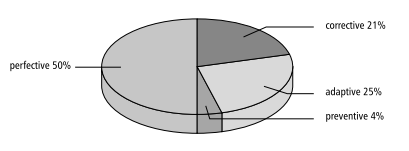
\includegraphics[width=0.8\textwidth]{images/maintenance.png}
	\caption{Distribution of maintenance activities\cite{Vliet:2008:SEP:1481475}}
	\label{fig:maintenanceActivities}
\end{figure}



%%%%%%%%%%%%%%%%%%%%%%%%%%%%%%%%%%%%%%%%%%%%%%%%%%%%%%%%%%%%%%%%%%%%%%%%%%%%%%%%%%%%%%

			% SOFTWARE REUSE

%%%%%%%%%%%%%%%%%%%%%%%%%%%%%%%%%%%%%%%%%%%%%%%%%%%%%%%%%%%%%%%%%%%%%%%%%%%%%%%%%%%%%%
\section{Software Reuse}
Software reuse is the process of using existing software artifacts, or knowledge, to create new software, rather than building it from scratch. Software reuse is a key method for improving software quality\cite{frakes1996software}. Software reuse can be specified in two directions, development \textit{for} reuse, and development \textit{with} reuse\cite{Slyngstad:2006:ESD:1159733.1159770}. Development for reuse is related to components for reuse or system generalization. Development with reuse is related to how existing components can be reused in new system.

Table \ref{tab:reusableComponents} lists several assets from a software project that can be reused\cite{frakes1996software}.
\begin{table}[H]
	\centering
	\begin{tabular}{ | l | l |}
	\hline
	1. architectures & 6. estimates \\ \hline
	2. source code & 7. human interfaces \\ \hline
	3. data & 8. plans \\ \hline
	4. designs & 9. requirements \\ \hline
	5. documentation & 10. test cases \\
	\hline
	\end{tabular}
	\caption{Reusable assets in software projects} \label{tab:reusableComponents}
\end{table}

Slyngstad et al.\cite{Slyngstad:2006:ESD:1159733.1159770} conducted an empirical study in Statoil ASA where their goal was to characterize developers views on software reuse. The results showed that reuse include lower costs, shorter development time, higher quality of the reusable components, and a standardized architecture. These findings are very similar to the key benefits of reuse that Lim has described\cite{lim1994effects}. The quality of software artifacts increases everytime the item is reused, because errors are discovered more frequently, making it easier to keep the artifact more stable\cite{sametinger1997software}.

Additionally, there can be problems associated with software reuse. A case study on a selected feature from self-driving miniature car development revealed that reuse of legacy, third party, or open source code, was one of the root causes for the accumulation of technical debt\cite{6974884}. Morisio et al.\cite{995420} idenfitied three main causes of software reuse failure; not introducing reuse-specific processes, not modifying nonreuse processes, and not considering human factors, combined with lack of commitment by top management.

%%%%%%%%%%%%%%%%%%%%%%%%%%%%%%%%%%%%%%%%%%%%%%%%%%%%%%%%%%%%%%%%%%%%%%%%%%%%%%%%%%%%%%

			% REFACTORING

%%%%%%%%%%%%%%%%%%%%%%%%%%%%%%%%%%%%%%%%%%%%%%%%%%%%%%%%%%%%%%%%%%%%%%%%%%%%%%%%%%%%%%
\section{Refactoring}
Design debt, a specific type of technical debt, accumulates as you write code\cite{Zazworka:2011:PDD:1985362.1985372}. This type of debt can be reduced when you refactor. Fowler defines refactoring as means of adjusting the design and architecture towards new requirements without changing the externial behaviour of a program in order to improve the quality of the system\cite{1999:RID:311424}. It is an act of improving the design of an existing system\cite{Vliet:2008:SEP:1481475}. Most of the time in spent on reducing design debt is on refactoring activities itself. These activities includes planning the design and architecture, rewriting the code, and adjusting documentation\cite{Pressman:2009:SEP:1593949}. It is believed that refactoring improves software quality and developer productivity, by making it easier to understand and maintain software codes\cite{Kim:2012:FSR:2393596.2393655}, thus a way to manage the technical debt of a system. 

Table \ref{tab:refactorArtifacts} lists the software artifacts that can be refactored\cite{1265817}.

\begin{table}[ht!]
	\renewcommand{\arraystretch}{1.2}
	\centering	
	\begin{tabular}{p{0.6\textwidth}} \hline
		\textbf{Programs} \\Refactoring at the source code or program level. For example, extracting methods, and encapsulating fields. \\ \hline
		\textbf{Designs} \\
		Refactoring at design level, for example in the form of UML models. Design patterns, software architecture, and database schemas, are some examples on artifacts that can be refactored at this level. \\ \hline
		\textbf{Software Requirements} \\
		Refactoring at the level of requiremetns specification. For example, decomposing requirements into a structure of viewpoints. \\ \hline
	\end{tabular}
	\caption{Types of Software Artifacts that can be refactored.}
	\label{tab:refactorArtifacts}
\end{table}


%%%%%%%%%%%%%%%%%%%%%%%%%%%%%%%%%%%%%%%%%%%%%%%%%%%%%%%%%%%%%%%%%%%%%%%%%%%%%%%%%%%%%%

			% CONFIGURATION MANAGEMENT

%%%%%%%%%%%%%%%%%%%%%%%%%%%%%%%%%%%%%%%%%%%%%%%%%%%%%%%%%%%%%%%%%%%%%%%%%%%%%%%%%%%%%%
\section{Configuration Management}
Systems always change to cope with bugs and introduce new features. A new version of a system is created when changes are made. Dart\cite{dart1991concepts} defines configuration management (CM) as a dicipline for controlling the evolution of software systems. CM identifies every component in a project and has an overview of every suggestions and changes from day one to the end of the product. CM involves four related activities\cite{Sommerville:2011:SE}:
\begin{description}
	\item[Change management] is intented to ensure that the evolution of a system is a managed process, and to prioritize changes. Costs and benefits has to be analyzed to approve changes and trach what components have been changed. The process starts with an actor submitting a change request. The request is checked for validity. If it is valid, the costs to this change are analyzed. The change request is passed to the change control board if it is not minor. The impact of the change from a strategic and organizational standpoint is considered, and if it is accepted, it is passed on. There are some important factors in the decision making process\cite{Sommerville:2011:SE}:\\
	\begin{inparaenum}[\itshape a\upshape)]
		\item The consequences of not making the change
		\item The benefits of the change
		\item The number of users affected by the change
		\item The costs of making the change
		\item The product release cycle
	\end{inparaenum}
	\item[Version management] is the process of keeping track of different and multiple versions of system components and ensuring that changes made to compoentns by different developers do not interfere with each other. This is often done with version management tools, which provide features like\\
	\begin{inparaenum}[\itshape a\upshape)]
		\item version and release identification;
		\item storage management;
		\item change history recording;
		\item independent development; or
		\item project support
	\end{inparaenum}
	\item[System building] creates an executable system by compiling and linking the program components, data, and libraries. The build process involves checking out component versions from the repository managed by the version management system, so it is necessary for system build tools and version management tools to communicate. There are many system build tools available, which provides features like 
	\begin{inparaenum}[\itshape a\upshape)]
		\item build script generation;
		\item version management system integration;
		\item executable system creation;
		\item test automation; or
		\item document generation.
	\end{inparaenum}
	\item[Release management] prepares the software for external release and keeps track of the system versions that have been released for customer use. Managing releases is a complex process as a release needs documentation such as configuration files, data files, and an installation program. Some factors that influences release planning are
	\begin{inparaenum}[\itshape a\upshape)]
		\item the technical quality of the system;
		\item platform changes;
		\item Lehman's fifth law;
		\item competitions;
		\item market requirements; or
		\item customer change proposals.
	\end{inparaenum}
\end{description}

There are some challenges related to development of embedded systems\cite{Estublier:2000:SCM:336512.336576}:
\begin{itemize}
	\item \textbf{Complex file sets}: Embedded systems consists of multiple diverse components, both hardware and software. This makes the system complex. Embedded system may also have different adjustable compoents for a specific platform, makin it easier to sell a product by tweaking some parameters. Dealing with these variates is a major challenge. Another challenge is that a product requires correct version of a component. Ensuring the consistency between components and their dependens files is a challenge as well.
	\item \textbf{Distributed teams}: Components may be developed in different places in our worl. Two team might for example work on the same components, especially when development are being outsourced. Such collaboration needs every developer to access each others work. The challenge is keep the team syncronized. 
	\item \textbf{Management and versioning of intellectual property}: Embedded systems, or software generally might use third-party technologies. It is important that those technologies are up-to-date, and maintained. These updates needs to be tracable such that each components has the right, compatible and stable version of its software. If something is not outsourced, it might be a challenge for developers to contribute and trace their changes.
\end{itemize}

Software CM (SCM) is the task of tracking and controlling changes in the software through reliable version selection and version control. SCM is a part of CM. Some examples on SCM that is widely used is Git, SVN, and Adele. Choosing a robust SCM system makes it possible to deal with big and complex files. It also supports distributed development. The right combination of SCM system and best practices makes it possible for embedded development projects to progress fast and efficiently. 



%%%%%%%%%%%%%%%%%%%%

% Kvalitet

%%%%%%%%%%%%%%%%%%%%%

\section{Software Quality}
Software Quality (SQ) is defined as \textit{an effective software process applied in a manner that creates a useful product that provides measurable value for those who produce it and those who use it}\cite{Pressman:2009:SEP:1593949}. The international standard for the evaluation of software quality presents six general properties that aims to give an overview of the software quality: functionality, reliability, usability, efficiency, maintainability, and portability. Table \ref{tab:qattribute} summarizes each quality attribute:

\begin{table}[ht!]
	\centering
	\begin{tabular}{ | l | p{8cm} |}
	\hline
	\textbf{Attribute} & \textbf{Description} \\ \hline
	Functionality 		& Ability of the system to do work for which it was intended. \\ \hline
	Reliability 		& Ability of the system to keep operating over time under certain conditions. \\ \hline
	Usability 			& The capability of the software product to be understood, learned, and used by users. \\ \hline
	Efficiency 			& The capability of the software product to provide appropriate performance, relative to the amount of resources used, under stated conditions. \\ \hline
	Maintainability 	& The capability of the software product to be modified in the future.\\ \hline
	Portability 		& The capability of the software product to be transferred from one environment to another. \\ \hline
	\end{tabular}
	\caption{Software Quality Attributes} \label{tab:qattribute}
\end{table}



%%%%%%%%%%%%%%%%%%%%%%%%%%%%%%%%%%%%%%%%%%%%%%%%%%%%%%%%%%%%%%%%%%%%%%%%%%%%%%%%%%%%%%
			
				% EMBEDDED SYSTEMS %

%%%%%%%%%%%%%%%%%%%%%%%%%%%%%%%%%%%%%%%%%%%%%%%%%%%%%%%%%%%%%%%%%%%%%%%%%%%%%%%%%%%%%%
\section{Embedded Systems}
%https://www.quora.com/What-are-the-characteristics-of-embedded-system

\textit{IEEE Standard Glossary of Software Engineering Terminology}\cite{radatz1990ieee} defines an embedded system as:
\begin{displayquote}
	\textit{A computer system that is part of a larger system and performs some of the requirements of that system; for example, a computer system used in an aircraft or rapid transit system.}
\end{displayquote}

While traditional computers are designed for performing multiple tasks, embedded systems are designed to perform a specific task under certain constraints. Embedded systems consists of small parts within a larger device that serves a more general purpose. For example, an embedded system in an automobile provides specific functions as a subsystem for the car itself\cite{Crnkovic:2005:CSE:1062455.1062631}. Due to their operational environment characteristics and common requirements, embedded systems are known as safety-critical and real-time systems\cite{563572,Crnkovic:2005:CSE:1062455.1062631}. This means that properties such as response time and worst case execution time are important design concerns\cite{4519555}: \textit{When the break pedal is pressed, the computer should initiate the breaking action within one millisecond}. A study of embedded systems shows that the various types of embedded systems share common requirements such as: \textit{real-time requirements, resource consumption, dependability, and life-cycle properties}\cite{crnkovic2004component}. It is expected that embedded systems are failure-free\cite{you2013reliability}, but these requirements might hinder embedded systems to deliver reliable service given a disturbance to its services, for example, failure in components\cite{patil2009embedded}. Additionally, it is expected that embedded systems has long life time\cite{563572}. Embedded systems are usually developed to deliver a service for long periods of time. Many of the embedded systems today were made many years ago, and thus have many weaknesses. 

Embedded software is defined as a computer software for embedded systems\cite{radatz1990ieee}. It includes the programs necessary to give functionality to the system hardware. As it runs on specialized type of hardware, embedded software has multiple contstrains related to run-time, memory usage, and processing power. Additionally, some other issues that needs to be addressed includes unstable requirements, technology changes, location of software errors, and inadequate documentation\cite{jimenez2013introduction}. In most cases, embedded software developers face many challenges in their work like conflicts in the requirements placed on them, for example, low memory usage while ensuring high availability\cite{vulgarakis2008embedded}. Moreover, old software are usually hard to maintain compared to new one, as they were made many years ago. Since embedded software has hardware constraints, companies must maintain many different configurations which makes maintenance a time challenge. Managing software quality is therefore necessary to deliver software in a useful, safe, and reliable way\cite{563572}. 





%Maintainability in embedded systems is as a property that allows the system to be acted upon, to guarantee a reliable operation thoroughout the end of its useful life\cite{introduction to embedded systems boka}. This property can be seen as a design constraint because it has to be planned from the project initiation. Large, expensive, and complex embedded systems are expected to remain in operation for decades, thus making maintenance an important property which allows reliable operation.

There are several challenges designers faces when it comes to integrating maintainability in embedded software. To improve the maintainability of embedded systems, some issues needs to be adressed, which includse unstable requirements, technology changes, location of software errors, hardware constraints, and inadequate documentation. Research has shown that addressing some of these changes improves the maintainability of embedded systems.


\subsection{Security}
Sommerville defines security as \textit{a systems ability to resist attacks. It is a complex property that cannot be easily measured. Attacks may be devised that were not anticipated by the system designers and so may defeat built-in safeguards}\cite{Sommerville:2011:SE}.
ISO 9126


\subsection{Dependability}




	% !TEX encoding = UTF-8 Unicode
% !TEX root = ../main.tex
% !TEX spellcheck = en-US

\chapter{Research Methodology}


%Architectural technical debt is a problem for many software projects today. Even though ATD is recognized in many studies, there is lack of focus on ATD in embedded systems. In this thesis, we will investigate how architectural technical debt can be identified in embedded software projects, and how it can be managed. This chapter describes the relevant research methods used in software engineering, and the methods that has been used in this thesis to answer the research questions. 

The nature of this thesis makes it suitable as an empirical research. To answer the research questions that was stated in Chapter 1, Section \ref{sec:chap1designquesitons}, an empirical research needs to be carried out in order to collect some data. This chapter provides a brief introduction to research methods in software engineering, and describes the research conducted in the thesis. Section \ref{sec:researchmethodsinsoftwareengineering} describes the relevant research methods in software engineering. Section \ref{sec:choiceofmethod} describes the research method that was chosen for this study. Section \ref{sec:researchprocess} presents the research process we have followed throughout this thesis, which includes our research design.





%%%%%%%%% SECTION RESEARCH METHODS IN SE %%%%%%%%%%%%


\section{Research Methods in Software Engineering}
\label{sec:researchmethodsinsoftwareengineering}
 Research is believed to be the most effective way of coming to know what is happening in the world\cite{bassey2003case}. Empirical software engineering is a field of research based on empirical studies to derive knowledge from an actual experience rather than from theory or belief\cite{empirical-research-SE}. Empirical studies can be explanatory, descriptive, or exploratory\cite{Wohlin:2000:ESE:330775}. 

 There are two types of research paradigms that have different approaches to empirical studies\cite{Wohlin:2000:ESE:330775}; the qualitative, and the quantitative paradigm. Qualitative research is concerned with studying objects in their natural setting\cite{Wohlin:2000:ESE:330775}. It is based on non-numeric data found in sources as interview tapes, documents, or developers' model. Quantitative research is concerned with quantifying a relationship or to compare two or more groups\cite{Wohlin:2000:ESE:330775}. It is based on collecting numerical data. 


To perform research in software, it is useful to understand the different research strategies that are available in software engineering. Oates\cite{Oates:2006:RIS:1202299} presents six different research strategies; survey, design and creation, case study, experimentation, action research, and ethnography. 

\textit{{Survey}} focuses on collection data from a sample of individuals through their responses to questions. The primary means of gathering qualitative or quantitative data are interviews or questionnaires. The results are then analyzed using patterns to derive descriptive, exploratory, and explanatory conclusions. 

\textit{{Design and creation}} focuses on developing new IT products, or artifacts. It can be a computer-based system, new model, or a new method. 

\textit{{Case study}} focuses on monitoring one single 'thing'; an organization, a project, an information system, or a software developer. The goal is to obtain rich, and detailed data. 

\textit{{Experimentation}} are normally done in laboratory environment, which provides a high level of control. The goal is to investigate cause and effect relationships, testing hypotheses, and to prove or disprove the link between a factor and an observed outcome. 

\textit{{Action research}} focuses on solving a real-world problem while reflecting on the learning outcomes. 

\textit{{Ethnography}} is used to understand culture and ways of seeing of a particular group of people. The researcher spends time in the field by participating rather than observing.




%%%%%%%%% SECTION OF OUR RESEARCH METHOD %%%%%%%%%%%%

\section{Choice of Research Method}
\label{sec:choiceofmethod}
The main purpose of this research project is to gain an understanding about the nature of technical debt in software design and architecture, and its potential sources in embedded systems in order to improve the management of software evolution. Based on the research questions stated in Chapter 1, we applied the case study approach to our research. Case studies provides both quantitative and qualitative information about the system\cite{Oates:2006:RIS:1202299}, depending on the approach the case study is taking.


\subsection{Case Study Method}
\label{subsec:casestudymethod}
%  Introduce methods, why. Design/plan, justify the why part.  Why this approach was chosen
Case study is an empirical method to investigate a single phenomenon within a specific time space in real-life context\cite{Wohlin:2000:ESE:330775}. Case studies excels at bringing an understanding of why or how certain phenomena occur or to add strength to what is already known through previous research\cite{Wohlin:2000:ESE:330775,soysusan}. Runeson et al.\cite{Runeson:2009:GCR:1519313.1519324} suggests case study as the most appropriate research method to use when exploring how a problem behaves in a real life context. In addition, they conclude that case study is suitable for software engineering research. There has been suggested systematic approaches for organizing and conducting a research successfully\cite{soysusan,Runeson:2009:GCR:1519313.1519324}. According to Yin\cite{yin2003case}, a research design is an action plan from getting here to there, where here is defined as the initial set of questions answered, and there is some set of conclusions about these questions. Moreover, a research design can be seen as a blueprint of research, dealing with at least four problems: what questions to study, what data are relevant, what data to collect, and how to analyze the results\cite{yin2003case}. Soy\cite{soysusan} proposes six steps that can be used when carrying out a case study:

\begin{enumerate}
	\item \textit{Determine and Define the Research Questions}: The first step involves establishing a research focus by forming questions about the problem to the studied. The researcher can refer to the research focus and questions over the course of study. 
	\item \textit{Select the Cases and Determine Data Gathering and Analysis Techniques}: The second step involves determining what approaches to use in selecting single or multiple real-life cases cases to examine, and which instruments and data gathering approaches to use. (whom we want to study, the case, cases, sample. and how we want to study it, design).
	\item \textit{Prepare to Collect Data}: The third step involves a systematic organization of the data to be analyzed. This is to prevent the researcher from being overwhelmed by the amount of data and to prevent the researcher from losing sight of the research focus and questions. 
	\item \textit{Collect Data in the Field}: This step involves collecting, categorizing, and storing multiple sources of data systematically so it can be referenced and sorted. This makes the data readily available for subsequent reinterpretation. 
	\item \textit{Evaluate and Analyze the Data}: The fifth step involves examining the raw data in order to find any connections between the research object and the outcomes with reference to the original research questions. 
	\item \textit{Prepare the Report}: In the final step, the researcher report the data by transforming the problem into one that can be understood. The goal of the written report is to allow the reader to understand, question, and examine the study.
\end{enumerate}

\section{Case Context}
\label{sec:casecontext}
% with whom /participants)One of the disadvantages using commercial is the constraints associated with obtaining permission to mine and publish findings.
To study the consequences of design debt, we have chosen to study a commercial system by conducting a case study. The conducted case study took place at Autronica Fire and Security AS, an international company with their headquarter based on Trondheim, one of the largest cities in Norway. Autronica is a leading innovator, manufacturer, and supplier of fire safety equipment and marine safety monitoring and surveillance equipment. AutroSafe, a high-end distributed fire alarm system, is one of the products they offer. The product was first released around year 2000, and has been on sale since. The product is mainly based of C/C++ source files. Project "Firmus" is the project name for the next generation AutroSafe. Firmus is a Latin word, which in English means: \textit{solid, firm, strong, steadfast, steady, stable, reliable, and powerful}. The goal with "Firmus" is to adopt newer technologies and technology standards that are used today. We had the opportunity to conduct our analysis on Project "Firmus". The project is still in the development phase. The goal of the analysis is to identify design debt before it gets worse. Table \ref{tab:systemmetrics} summarizes the system metrics, which includes the test files.

% Summary of system: Written in C/C++ and has been in development since late 1990s. It is used widely on their products. We have studied a pilot project which goal is to use better design, technologies etc. This is a pilot project so it has not entered the evolution. Our goal is to identify technical debt that has accumulated recently, and we'd like to discover them before they get messy. 

\begin{table}[]
\centering
\caption{System Metrics}
\label{tab:systemmetrics}
\begin{tabular}{|l|l|}
\multicolumn{2}{c}{\textbf{Project Firmus}} \\
Lines                      & 88465          \\
Lines of Code              & 49287          \\
Lines of Comments          & 23017          \\
Components                 & 13             \\
Files                      & 461            \\
Number of Classes          & 339           
\end{tabular}
\end{table}

As we mentioned, the product is mainly based of C/C++ source code files. The software architecture of the Project "Firmus" is component-based, where the different source files are divided into each their component. In total, the system consists of 13 components, and 461 source code files. To ensure reuse of code and libraries, the company has developed a library that is used by this system and other systems as well.


\section{Research Process}
\label{sec:researchprocess}
A research process provides a systematic approach on how to fulfill the goal of a research. In this study, we have chosen to follow the principles of the six steps defined by Soy\cite{soysusan}: \textit{Determine and Define The Research Questions, Select the Cases and Determine Data Gathering and Analysis Techniques, Prepare to Collect Data, Data Collection, Evaluate and Analyze Data, and Prepare the Report}.

%FIGURE:

%1 {Experiences and Motivation -> RQ} -> 2 {Case Study, Documents, Qualitative, Type: Descriptive and Exploratory} -> 3 {Prepare, organize and structure the data (ISO 9126 for requirements)} -> 4 {Data collection} -> 5 {Data analysis} -> 6 {Findings, conclusion, report,  All steps and methods that has been conducted during the the research will be reported through this thesis. }

\subsection{Determine and Define the Research Questions} % Pre study, state of the art
First, we need to set up the goals of this research by defining the research questions. In prior to our previous research\cite{forprosjekt}, we stated that we are interested in getting deeper insight into the field of technical debt. As mentioned in Section \ref{sub:classificationtechdebt}, many subcategories of technical debt exists. With regards to that, we have chosen to investigate design debt in embedded systems.

In order to determine and define the research questions, we begin with an analysis of the state-of-the-art to determine what prior studies have determined about the topic of software design flaws. Google Scholar, ACM Digital Library, Scopus, and IEEE Xplore Digital Library were used tremendously in order to gather research papers for the analysis of the state-of-the-art topics that are relevant for our thesis. After getting familiar with the topics of area of this study, we defined our research questions for this study. These research questions will be our primarily driving force thorough this research. We have defined four research questions RQ1-4, which we have summarized in Table \ref{researchQuestionsChapter3}.

\begin{table}[]
	\centering
	\caption{Research Questions}
	\label{researchQuestionsChapter3}
	\begin{tabular}{|l|p{8cm}|}
		\hline
		\textbf{RQ1} & How can design debt be identified?     \\ \hline
		%\textbf{RQ2} & Why does design debt accumulate? \\ \hline
		\textbf{RQ2} & What are the effects of design debt?  \\ \hline
		\textbf{RQ3} & What kind of design debt can be found in embedded systems? \\ \hline
		\textbf{RQ4} & How to pay design debt? \\ \hline
	\end{tabular}
\end{table}



\subsection{Select the Cases and Determine Data Gathering and Analysis Techniques} % Case Context
%This study addressed the research questions. Furthermore, we gathered data by analyzing documents and code. %Additionally, interviews were used to get a deeper insight about the problems from the developers.
To investigate the research questions, a representative context has to be chosen. With regards to that, we have chosen to conduct an exploratory and descriptive case study in real-life context to obtain knowledge about the problem to be studied. The case study took place at Autronica Fire and Security AS for approximately six weeks. A brief description of the company can be found in Section \ref{sec:casecontext}. Autronica provided us a workspace and multiple data sources, including access to their source code, issue lists in Stash, system requirements, and design and code documentation. Our data were mainly extracted from these sources.

A part of the literature review was to get familiar with existing tools that has been used to address similar problems. Below, we have listed each tool that has been used to extract relevant data in this case study. Doxygen is used by the company to generate and keep the documentation up-to-date. In order to understand the system and how the different components interact, we spent some time analyzing the system documentation. Moreover, Doxygen can generate various diagrams such as inheritance diagrams, and dependency graphs. However, a downside with Doxygen is that it lacks a feature for interacting with the diagrams and graphs. Doxygen allows us to specify depth of the graphs that are generated, but they can become very large, which makes the graphs difficult to understand. Moreover, Doxygen does not provide full diagrams for internal dependencies in each component, it can generate dependencies for a chosen file. There are many tools that offers reverse engineering of C/C++ source code, so we decided to try out a few of them, including ArgoUML, Enterprise Architect, and Understand. 

Some static analysis tools has been used to extract design problems at code level. These includes Understand, SonarQube, CppClean, CppDepend, CppCheck, and Sonargraph. 

\subsubsection{Selection of Tools}
Various tools have been used to mine for data and understand the structure of the system studied. The following sections will describe the tools that has been used in this research.

% Kilde: http://www.stack.nl/~dimitri/doxygen/
\textbf{Doxygen} is a free software for generating documentation from annotated C++ sources. Doxygen has the ability to generate documentation in HTML or in Latex. Since the documentation is extracted from the source code, it is easier to keep the documentation up to date. In addition, Doxygen can be configured to extract the code structure from undocumented sources files, which makes it possible to visualize the relations between various elements in the software. Doxygen is used by the company to keep the documentation up-to-date, and was therefore used in this project to learn about the system and to visualize the system.

\textbf{ArgoUML} is an open source UML modeling tool that includes support for all standard UML 1.4 diagrams\cite{argouml}. ArgoUML features reverse engineering of C++ projects by reading C++ source files and generate and UML model and diagrams. 

\textbf{Enterprise Architect} is a commercial UML modeling tool. It has the ability to produce UML diagrams from code. This tool was used to create class diagrams for each component, allowing us to identify possible code smells, such as Large Class code smell, and God Classes.

\textbf{SonarQube} is an open source platform for quality management of code. It has the ability to monitor different types of technical debt. It supports multiple languages through plugins, including Java, C/C++, JavaScript, and PHP. A downside with SonarQube is that some of the plugins requires a commercial license, and that some features included are not applicable for C++.

\textbf{Understand}  is a commercial code static analysis tool. It supports dozen of languages, including Java, C/C++, Fortran and Python. Understand can help developers analyze, measure, visualize, and maintain source code. It includes many features, including dependency graph visualization of code, and various metrics about the code (e.g. coupling between object classes),. 

\textbf{CppDepend} is a commercial static analysis tool for C/C++ code. 

\textbf{CppClean} is an open source static analysis tool for C/C++ code. It attempts to detect problems in C++ that slow development in large code bases. Among many features, CppClean supports finding unnecessary \textit{'\#includes'} in header files, global/static data that are potential problems when using threads, and unnecessary function declarations.

\textbf{CppCheck} is another open source static analysis tool for C/C++ code. Unlike CppClean, CppCheck detects various kinds of bugs that the compilers normally do not detect, such as memory leaks, out of bounds, and uninitialized variables.

\textbf{CCCC} is a free software tool for measurement of source code related metrics. This tool are able to measure some of the metrics that are defined by Chidamber and Kemerer\cite{chidamber1994metrics}.

\textbf{SourceMonitor} is a program which inspects the source code to find out how big the system is and to identify the relative complexity of the modules. It collects metrics through source files.

Data is collected from issue lists, and has been mapped to their corresponding components and source files in order to find which component we should look more at. This data will be compared to the data we have extracted using static analysis tools mentioned above.


\subsection{Prepare To Collect Data}
The third step in this case study is about preparing for data collection. Firstly, we need to review the system documentation in order to get familiar with the system and its components. Due to the time limit, we have chosen to collect data from three critical components using the tools listed in Section XX. We prioritize the components using the issue lists, and break down the components to identify bad design. Bad design includes god classes, dependency cycles, complex interfaces, and unused code in the components. A Word document is created to keep track of the extracted data so we can review it later for analysis. If any interviews would be needed, they would be set up and planned on this stage. 


\subsubsection{Metrics Selection}
Using Understand, we measured the software metrics by analyzing the source code. In total, we extracted 9 metrics for each class on the system, excluding the tests.

\begin{itemize}
	\item LCOM (Lack of Cohesion in Percent): A method is cohesive when it performs a single task. Low cohesion increases complexity, and will increase the likelihood for errors during development process. In general, the desirable value for LCOM is to be lower. 

	\item DIT (Max Depth Inheritance Tree): The longest path from a given class to the root class in the inheritance hierarchy.

\item CBO (Coupling Between Object classes): Number of other classes that are coupled to this class. Desirable value is lower. 

\item NOC (Number of Children): Number of subclasses from a given class.

\item RFC (Response For a Class): The sum of the number of methods that can be potentially executed in response to a message by an object of a class.

\item NIM (Number of Instance Methods): Number of instance methods in a class, which is methods that are accessible through an object of that class.

\item NIV (Number of Instance Variables): Number of instance variables in a class, that is, variables that are only accessible through an object of that class. This variable is used to measure LCOM values. In addition, it can be used to identify God Classes.

\item WMC (Weighted Methods per Class): The number of all local methods in a class. More member of functions is considered to be more complex and therefore more error prone. Desirable value is low.

\item WMC2 (Weighted Methods per Class 2): This metrics sums the cyclomatic complexity of each class by counting the cyclomatic complexity for each method.
\end{itemize}


For each metrics, we have computed descriptive statistics on all the classes of the system. These statistics aims to give a measure of the value of the metrics for all the classes, which we can use to identify classes with weak metric values. These statistics are:

\begin{itemize}
	\item Minimum: The minimum value of a metric.
	\item Maximum: The maximum value of a metric.
	\item Sample Mean: The mean of the metric, that is, the average value of a metrics. It can be used to measure the center of the data.
	\item Median: Value in the middle of a given data set.
	\item Standard Deviation: A measure of how spread out the numbers are. Higher values indicates greater spread.
\end{itemize}



% How is data collected, from where
\subsection{Data Collection}
The fourth step of the research process is to execute the plan that was created in step three. During the case study, data is collected from two different sources by using multiple tools to improve the reliability of the study. The first source of design flaws it to identify for code smells in the source code. Table \ref{tab:codesmell} in Section \ref{subsub:codesmell}, Chapter 2, summarizes the code smells that are presented by Fowler et al.\cite{fowler1999refactoring}. By using automatic static analysis tools, we were able to identify multiple code smells in the system. Most of the code smells were manually verified by the researcher by inspecting the class and dependency diagrams for the class in which code smell exists. For instance, Duplicated Code code smell were identified using SonarQube. We inspected each file with duplicated code to verify the results. Another example of a code smell we identified is the Long Method code smell. Long Method code smell was identified using CppDepend and Understand. The results were verified by reverse engineering the source code to generate UML class diagrams. At first, we used the built-in functionality in Doxygen to generate the class diagrams. However, Doxygen was not able to provide full class diagrams. Therefore, we had too look for other options. We came across ArgoUML, an open source alternative to generate UML diagrams by reverse engineering C/C++ code. After comparing some of the results with snippets from Doxygen class diagrams, we noticed that ArgoUML failed to reverse engineer some of the classes and their corresponding relations to other classes. This led us to look for commercial software. Using Understand, we were able to extract the class diagrams for the system by using their built-in reverse engineering functionality. UML class diagrams were also used to verify Large Class code smell and God Classes. In addition, a dependency graph was extracted, which show internal dependencies in each component, and dependencies between components. We noticed two form of dependencies, direct dependencies and circular dependencies. 

The second source of design flaw extraction identification is to measure the object-oriented metrics for the system. Object-oriented metrics are used to manage, predict, and improve the quality of a software product\cite{rodriguez2001overview}. Using Understand, CCCC, and SourceMonitor, we were able to extract multiple metrics. More precisely, we have extracted the following metrics: LCOM, DIT, CBO, NIV, NIM, WMC, NOC, and WMC2. In our measurements, we decided to exclude the test classes as they may affect the metrics in both positive and negative way.




\subsection{Evaluate and Analyze the Data}
In the fifth step of the case study, we will examine the data collected in fourth step. For the data analysis of the collected object-oriented metrics, we perform some statistical analysis by measuring the descriptive statistics for the different metrics. Descriptive statistics are used to summarize data in a meaningful way. By examining the data, we may be able to identify some patterns in the data. The descriptive statistics we have measured are the following; minimum, maximum, median, sample mean, and standard deviation. The minimum and maximum value helps us to identify the smallest and largest data value in the data set. The median value is the midpoint of the data set. It helps us identifying which half of the observations are above and below the midpoint. Sample mean is the average of the data, which is found by summing all of the observations divided by the number of observations. Both median and sample mean measure the central tendency. At last, the standard deviation measures how spread out the data are from the mean. Higher values indicates greater spread in the data. Furthermore, we calculate the frequency distribution for the different metrics. This was done to make the findings more accessible by visualizing the data, and to interpret the data afterwards. The results are then compared with some of the defined thresholds in the literature, and our findings from the literature review. 

For the analysis of the code smells we have detected, we have manually inspected some of the detected smells in order to determine whether the hits are false negative or false positive. 



\subsection{Prepare the Report}
At last, the methods conducted will be reported through this thesis. This involves all the steps that we have gone through this thesis, including stating the problem, performing a literature review, listing the research questions, explaining data gathering and analysis techniques used, and a conclusion where research questions are answered and suggestions are made for further research. The report also includes findings from the literature review, and how they are related to our findings from the case study. At last, the report conclusion makes suggestions for further research, so that other researchers may apply these techniques in some other context to determine whether findings are similar to our research or not.


\section{Summary of the Research Design}
The research questions described in Section XX were answered using the case study methodology and a literature review. The literature review helped us getting familiar with the topic and to identify the tools needed to mine data. Furthermore, the case study was conducted in collaboration with a company located in Trondheim. 



























	% !TEX encoding = UTF-8 Unicode
% !TEX root = ..\main.tex
% !TEX spellcheck = en-US
\chapter{Results}
This chapter presents the results of this study. The first section presents the participants. The main findings are presented in Section \ref{sec:techDebt}, \ref{sec:techCause}, \ref{sec:prior}, and \ref{sec:managing}. Section \ref{sec:techDebt} focuses the term TD and causes related to it. Section \ref{sec:techCause} reveals the causes of TD. Section \ref{sec:prior} takes a further look at how TD is addressed and prioritized in organizations. Section \ref{sec:managing} reveals the way TD is managed.

% Bakgrunn
\section{Introduction of participants}
\label{sec:background}

\begin{table}[ht!]
	\centering
    \begin{tabular}{|p{1cm}|p{4cm}|p{4cm}|p{4cm}|}
    \hline
    \textbf{ID} & \textbf{Role} & \textbf{Academical degree} & \textbf{Experience}    \\ \hline
    P1 & Software Developer               & Bachelor          & Over 10 years \\ \hline
    P2 & ICT Security and Quality Manager & Master            & Over 10 years \\ \hline
    P3 & Research and Developer Manager   & Doctoral          & Over 10 years \\ \hline
    P4 & Project Manager                  & Doctoral          & Over 10 years \\ \hline
    \end{tabular}
    \caption{The participants and their background} \label{tab:participants}
\end{table}

The participants had various background within software development field. As mentioned in Chapter 3, two of the participants works with embedded systems, and the last two works with traditional software development. Table \ref{tab:participants} summarizes their background.

The interview began by asking the participants about their responsibilities with the products they are working on, type of products they develop, size of the product, size of the projec team, and software development methodology used. Table \ref{tab:participantsResponsbilities} summarizes their responses.

\begin{table}[ht!]
	\centering
    \begin{tabular}{|p{0.5cm}|p{2.5cm}|p{3.5cm}|p{2cm}|p{2cm}|p{2cm}|}
    \hline
    \textbf{ID} & \textbf{Product type} & \textbf{Responsibilities} & \textbf{Size of the solution (lines)} & \textbf{Process} & \textbf{Team size}\\ \hline
    P1 & Web application & Working on an API, integrates multiple systems & 101k - 1m & Scrum & 5 to 10 \\ \hline
    P2 & ERP solution, SAP project & Maintains and manages systems & More than 10m & Lean, Scrum & More than 20 \\ \hline
    P3 & Embedded systems & Creates products by integrating other products with their own core product & 101k - 1m & Lean, Scrum & 11 to 20\\ \hline
    P4 & Embedded systems & Project leader, creates COTS solutions & 101k - 1m & Scrum & More than 20 \\ \hline
    \end{tabular}
    \caption{The participants and their project} \label{tab:participantsResponsbilities}
\end{table}






% Om teknisk gjeld

%The interviews started by asking the participants what their definition of technical debt is, what the causes for technical debt were, and why technical debt is a problem today. 
\section{Definition of Technical Debt}
\label{sec:techDebt}
To get an understanding of what the participants meant when they talked about TD, they were asked to define the term.
\begin{displayquote}
\textit{"Technical debt is resolving things in a way so that there will be need of refactoring the solution later. Technical debt is incurred intentionally or unintentionally. It may be due to external assumptions that were not taken into account when designing the system. You can have the perfect payment system, but if you change the currency, the system may fail."} - P1.  
\end{displayquote}

P2 defines TD as follows:
\begin{displayquote}
\textit{"Systems or software that performs under the level we have set as requirement, or is of lower quality. Like if we have systems out-of-support, then we have incurred technical debt as the system operates with bigger risk than what we want. [...] We do not want to run the latest version of a software, but a version less because someone has run it before and fixed the bugs."} - P2.
\end{displayquote}

The definition of TD given by P3 is:
\begin{displayquote}
\textit{"A product where components are not available, operating system is outdated and is not supported with updates anymore. It is expensive to maintain the product, and people with the competence might not be available anymore."}.
\end{displayquote}

P4 defines TD as \textit{"things that needs to be changed before you can add new functionality"}.

\subsubsection{Why TD is a problem}
The literature stated that TD is not always bad\cite{p31-guo}. With that in mind, the participants were asked why they consider TD as a problem. Both P2 and P3 explained that incurring TD resulted in long-term risks. 

\begin{displayquote}
	\textit{"Technical debt is a problem because all the products we deliver, will incur technical debt, if developers do not care to maintain the product, and remove unhealthy dependencies along the way that you quickly get as a result of technical debt. Another problem is that people are afraid to bring up this subject. I talked with a guy from the oil sector who told me that some of their systems has 40 years of technical debt. I think that it is time for an upgrade. The world has changed radically over the past decade and will change in the future."} - P3.
\end{displayquote}

P2 expressed that their organization have many legacy equipments and systems. Additionally, their systems are using legacy technologies. Legacy solutions creates troubles in the long-run. \textit{"An example of a system we have running on Windows 95, cannot be upgraded or replaced due to compatibility problems. You cannot install Windows 95 on a new PC, because Windows 95 will not understand the drivers that the new PC needs. There are many organizations that keeps buying systems without having a plan for how to manage it later"} - P2. 

%It is expensive to change the system because the code might not work on newer systems. The code might not be compatible with newer systems either. These types of problems creates security breaches, as you are not able to upgrade and update the system. 

P4 explained that there is always a possibility of refactoring in projects. \textit{"Our code base is almost 10 years old, and big parts of the architecture is still the same as it was 10 years ago. I am pretty sure that there are some parts of the system that can be improved"} - P4. 

P1 remarked that TD is now always bad.
\begin{displayquote}
\textit{If you create systems that does not incur technical debt, there would not be so much for developers to do later. This is the reason for agile methods being used, you create visible technical debt. Your boss might give you a task to build a house without a roof. The house looks very nice, but the day it snows, things will go bad} - P1.
\end{displayquote}






\section{Causes of Technical Debt}
\label{sec:techCause}
%Hvorfor de tror TG oppstår generelt. Kan si noe om eksempler fra de ulike scenarioene
To identify the causes of TD, the participants were asked the reasons for TD accumulation in their project.

\subsection{Time Pressure}
Time pressure was frequently mentioned as a reason for incurring technical debt. For example, P1 and P4 mentioned that if they did not incur technical debt, it ran the risk of not being able to deliver the solution at all. 

\begin{displayquote}
\textit{"Sometimes, we need to take shortcuts in order to meet a deadline. We do not take shortcuts in terms of bad code, but rather to complete functionality and integrate them into our solution. Less important tasks can be postponed."} - P4.
\end{displayquote}

Furthermore, P2 explained that both lack of time and resources is why technical debt keeps growing in their systems. He explained that the resources they are given by the management are mostly used to implement new functionality, or to fix critical errors. They do not have the time to upgrade their existing systems.
\begin{displayquote}
\textit{"We cannot prioritize upgrading existing systems. The resources that are given to us, are used to implement new functionality, or to fix critical errors such as system crashes. It is not certain that technical debt is behind a system crash, but it is something we need to prioritize. Additionally, we get new projects all the time, which makes software evolution a challenge."} - P2.
\end{displayquote} 
Moreover, P2 mentioned that one of their systems did not work properly after upgrading the operating system it was running on. Given the lack of resources to pay down TD, they eventually had to isolate the problem by workarounds. 

\subsubsection{System Size}
As the system complexity keeps increasing, the system also becomes harder to change. Increased system complexity makes it easier and cheaper to incur TD in short-run. P4 explained that many of their developers did not know the system well enough, so change requests made by developers did not fit with the intended design.

\subsubsection{Architectural Decisions}
Furthermore, P1 revealed a situation where an architectural decision was the reason for TD accumulation. The solution looked good to begin with, but the effects of the outcome was not optimal. The architecture design was a debt itself. He further stated that while the implementation was good, the outcomes was not as expected.

\subsubsection{Technology Choices}
The participants explained that technology and framework choices, may be a source of technical debt. Both technologies and frameworks gradually become obsolete by other solutions, resulting in legacy. P3 described a situation where their core product accumulated technical debt over time. The product used lots of legacy solutions from external suppliers. Replacing these was expensive because it would require changes at the infrastructure level of the system. However, at some point, the organization decided to manage the technical debt by re-engineering the solution using open-source solutions.




\section{Incurring Technical Debt}
\label{sec:prior}
%P1 and P2 revealed that requirements from the management or customers are the dominant factor in determining if the available resources should be used to address technical debt, while deadlines are the dominant factor. 
The participants were asked about the current level of technical debt in their products, and the reason for it. Both P1 and P2 revealed that requirements from the management or customers are the dominant factor in determining if the available resources should be used to address technical debt, while deadlines are the dominant factor for P4. 

\begin{displayquote}
\textit{"There are some visible and some invisible technical debt in our project. Mostly visible that should have been fixed. The reason for it is that the product is relatively new and young, which makes it more important to deliver new functionality."} - P1
\end{displayquote} 

P2 explained that they have accumulated lots of technical debt in their product, both known and unknown. Their product consists of outdated solutions from external suppliers. They usually fix errors by workarounds, resulting in architecture violations. Legacy components are hard to change. Another problem that was mentioned is that there is no documentation or knowledge about the components, hence making it difficult to change the internal structure of the solutions.

However, the product P3 is currently working on has accumulated small amounts of technical debt. The reason is that the product is relatively new. Their previous solution of the product had accumulated a high amount of technical debt. They ended up replacing the old solution with a new, improved solution using open-source technologies. Furthermore, P3 stated that shortcuts are taken if they need to reach a deadline. However, they always makes a plan to address it in the future. Test-driven development is used a lot thorough the development, making sure that problems are addressed immediately.

P4 remarked that they have accumulated some technical debt in their product, but not more than they are able to handle. Most of the technical debt they have accumulated are related to integration and system tests. P4 also stated that technical debt is not bad. Sometimes, technical debt needs to be incurred, to meet business goals. \textit{"You can take a loan from the bank to buy a house, as long as you are able to pay it back"} - P4.

Some of the participants revealed that TD is incurred intentionally to a certain extent. P1 explained that both developers and the management makes such decisions. 
\begin{displayquote}
    \textit{"Developers tries simple solution to understand the exact problem. They usually hard code some parts of the code that could have been coded dynamically. However, hard coding results in short-term benefits, but it causes long-time problems." - P1}
\end{displayquote}


\subsubsection{Short-term vs. long-term effects}
The interviews revealed that technical debt may affect the software development in the short-term. Incurring technical debts by taking shortcuts, is used to save development time and deliver a solution faster to the customers. P4 explained that technical debt is not the result of poor programming skills, but as a result of intentional decisions to trade off competing concerns during development. P1, P2, and P4 mentioned that such shortcuts in development are taken, in reaction to business pressure. Another short-term effect of technical debt that was identified is the customer satisfaction. The customers are interested in getting the product on time. They do not care about the technical details of implementation as long as it does not directly affect the product quality. \textit{"The customers does not care how they get electricity from the wall, they just want electricity" - P2}. Moreover, P4 mentioned that sometimes short-term solutions might outweigh the future costs, depending on the implementation method.

The negative effects tended to be on the longer term, such as poor performance, increased complexity, and low maintainability. P3 brought up example where one of their systems that used legacy technologies, crashed during a scaling test. P2 mentioned that some of their systems are still running on Windows 95, and they do not have enough resources to upgrade the systems. Both P1 and P2 mentioned that TD is also incurred intentionally. Management and the customers often comes with requirements that needs to be prioritized. 

\begin{displayquote}
    \textit{"Lets say that we have two systems with technical debt. If we have resources to manage technical debt in one of the systems, the other system needs to be postponed. These types of situations occurs frequently, and the total technical debt keeps increasing." - P2}
\end{displayquote}


% Hvor mye som investeres for å måle kvalitet
\subsubsection{Prioritizing Technical Debt}
Another aspect with software development we found interesting is how business decisions affects the development team and the overall software quality. With regards to that, the participants were asked about to what extent the company invest resources to measure the quality of the system.

Both P1 and P2 mentioned that business decisions do have effect on the amount of technical debt. 
\begin{displayquote}
\textit{"Customer specified functionality have to be prioritized for business purposes. Such decisions often causes architectural erosion. The software may work, but the solution is dirty.""} - P1
\end{displayquote}

\begin{displayquote}
\textit{"The management is not willing to see what people are doing during work, and how much time it takes to finish a task. This leads to problems in distribution of resources.""} - P2
\end{displayquote}

P1 further mentioned that there is a communication gap between the team and the management. \textit{Not everyone from the management is known with the term technical debt. If something works, do not touch it - P1}.

P2 explained that the management is interested in the risks behind technical debt issues, before taking a choice. Management do not care about the consequences if the risk is low, as long as it does not have any big impacts for the business. 

P4 remarked that the quality on their product is remarkable. He stated that it is hard to measure the quality of their product, so they use feedbacks and reviews from the customers as a way to measure the quality.

\section{Management of Technical Debt}
\label{sec:managing}
Another important aspect regarding TD is how it is managed. The participants were asked about the importance of reducing TD, and how they reduce TD. Most of the responses involved some form of communication within the development team, and with management. It included approaches such as risk management, and use of backlogs. Some of the participants also pointed out that TD can be controlled by the customer, based on the needs.

% How important is it to reduce TG
\subsubsection{Importance of reducing TD}
A common response regarding the importance of reducing TD is the products ability to remain stable.

\begin{displayquote}
\textit{Managing technical debt by upgrading the software is not necessary a goal, it is more important to use a version of the software that is stable.  A small change in the software may affect many people. [...] It is important to finish a task early as possible, and to clean up the mess before you end up with too much dependencies} - P1
\end{displayquote}

However, reducing TD is a challenge itself. P3 commented that the challenge is to get project leaders attention on various problems. \textit{"Sometimes, there is need of refactoring technical debt. Postponing technical debt problems create long-term issues. A challenge is to get an approval from the project manager to address the issue. It is important to fix technical debt problems while it is fresh. Keep the code agile."} - P3. 

Furthermore, the participants were asked how much time the team spent on reducing TD. P3 and P4 remarked that fixing software bugs is something they work with all the time. The goal is to get an overview of all the bugs before product shipment to customers. P4 stated further than bugs are not considered as TD. TD is code that needs refactoring. P1 and P2 handled TD in parallel with development of new functionalities. Both of them spend around 25\% to 30\% each sprint on maintenance and evolution.


%What tools and techniques are used to manage it
\subsubsection{Tools and techniques}
The participants stated different ways to handle TD. rRefactoring and re-engineering were commonly mentioned. P3 had to re-engineer the core of their product using open-source software. Additionally, various tools are used to keep track of the TD. The most common mentioned tools was Jira, and issue trackers. However, one of the participants commented that they do not have any special tools for TD management. 

\begin{displayquote}
	\textit{We do not use any special tools or techniques to manage TD. We do have a system- and a service catalog. These catalogs gives an overview over all the systems we are working with. It displays information such as hardware and software version that is used, and age of the system. Administrators use these catalogs to create tasks for the different projects that are on-going. If some software or hardware is very old, the issues are addressed by risk management} - P2.
\end{displayquote}

P3 considers TD issues all the time thorough the development. By using test driven development, they are able to address TD issues relatively fast. However, issues are raised if it is something important. Their goal is to fix it the next release.  

%How they would like to manage technical debt.
The participants were asked how they would like to manage TD. P1 mentioned that encapsulating the code might help in the short-term. Software architecture does not get affected by encapsulation. Raise an issue, and put it on the backlog. Fix it the next sprint. Both P2 and P3 would like to use a fixed budget for managing TD. Using the budget, they would prioritize the tasks based on what effects it has for the customer. \textit{"Systems are getting older and older each day, and the quality is getting worse. You should think about replacing it" - P3}. P4 would like to spend more time on managing TD on each sprint. Ideally, 20\% of the time on each sprint.



	% !TEX encoding = UTF-8 Unicode
% !TEX root = ..\main.tex
% !TEX spellcheck = en-US

\chapter{Discussion}
This thesis aims to investigate the possibilities to identify design debt in embedded systems. Our case study evaluated a software system written in C/C++. This chapter will discuss the results we gathered during our case study. Section 5.1 contains a discussion the measured values for object-oriented metrics by applying a set of threshold values to uncover possible unsecure parts of the code. Section 5.2 will lo



\section{Evaluation of Object-Oriented Metrics by Applying Threshold Values}
Measuring software metrics in object-oriented software is important in terms of quality management\cite{tarcisio,ferreira2012identifying}, as software metrics can be used as predictors of fault-prone classes in object-oriented systems\cite{basili1996validation}. A study by Basili et. al\cite{basili1996validation} assessed Chidamber and Kemeerers\cite{chidamber1994metrics} suite of object-oriented metrics as predicators of fault-prone classes. Their results implied that object-oriented metrics appear to be useful to predict class fault-proneness during early phases in software life-cycle. Object-oriented measurements alone are not necessary sufficient to identify parts of the system with major design violations. According to Tarcisio, software metrics are not effectively used in software industry due to the fact that for the majority of metrics, thresholds are not defined\cite{tarcisio}. Threshold is defined as values used to set ranges of desirable and undesirable metric values for measured software\cite{ferreira2012identifying}. Knowing thresholds for metrics allow us to assess the quality of a software, and we may be able to identify where in a design errors are likely to occur. Lanza et al.\cite{lanza2007object} presents two ways to identify major sources for threshold values; statistical information (i.e., thresholds that are based on statistical measurements), and general accepted semantics (i.e., thresholds that are based on information which is considered common).  

Threshold values were derived for the individual metrics using their descriptive statistics from Table \ref{tab:oometrics-firmus} in order to identify the classes with major design violations. Threshold values have been identified using statistical information\cite{lanza2007object}. For each metric, we used the the sample mean and standard deviation from Table \ref{tab:oometrics-firmus} to derive its corresponding threshold value. The first threshold value is corresponds with the mean and represents the most typical value in the data set\cite{cais2014identifying}. According to Lanza et al.\cite{lanza2007object}, the first threshold value can be calculated by subtracting the standard deviation from the sample mean. However, the standard deviation in our data set may be larger than the sample mean, which leads to negative threshold values. The second threshold value the sum of the sample mean and the standard deviation. It represents high, but still acceptable values. The third threshold value is simply the second threshold value multiplied with 1.5\cite{lanza2007object}. It is considered as extreme, and should not be included in the data set. In addition, we have gathered thresholds that has been proposed by researchers for the metrics we have measured in this thesis. Table \ref{tab:thresholds} presents the metrics and their threshold values.

\begin{table}[ht!]
\resizebox{\textwidth}{!}{
\centering
\caption{Thresholds for object-oriented software metrics}
\label{tab:thresholds}
\begin{tabular}{|l|p{2cm}|p{2cm}|p{2cm}|p{2cm}|p{3cm}|}
\hline
\textbf{Metric} & \textbf{Observed Value} 	& \textbf{Low} 		& \textbf{High}  & \textbf{Extreme value} 	& \textbf{Recommended Max Value} \\ \hline
LCOM   			& 100			         	& 42				& 75   			 & 100+						& 72.5\cite{tarcisio}           \\ \hline
DIT 			& 4             			& 1					& 2				 & 3+						& 4\cite{tarcisio}, 5\cite{rosenberg1999risk,metricoverview,metricsguide}              \\ \hline
CBO    			& 30  			          	& 6					& 11			 & 17+						& 5\cite{rosenberg1999risk,metricsguide}, 14\cite{sahraoui2000can,phpdepend}     \\ \hline
NOC    			& 20 			           	& 0					& 2				 & 4+						& 3\cite{tarcisio}, 5\cite{metricsguide}, 10\cite{metricoverview}               \\ \hline
RFC    			& 115           			& 15				& 34			 & 51+						& 50\cite{rosenberg1999risk}      \\ \hline
NIM    			& 48            			& 8					& 15			 & 23+						&               \\ \hline
NIV    			& 18            			& 2					& 5				 & 7+						&             \\ \hline
NOM    			& 48            			& 9					& 16			 & 24+						& 20\cite{rosenberg1999risk}                \\ \hline
WMC    			& 325  			         	& 19				& 51			 & 76+						& 34\cite{tarcisio}, 40\cite{rosenberg1999risk}, 50\cite{phpdepend}      \\ \hline
\end{tabular}}
\end{table}


For 101-1000 classes:

CBO: Good: 0-1, regular: 2-20, bad: 20+
NIV: 0-1, 1-8, 8+
NIM: 0-25, 6-50, 50+
DIT: 2
LCOM: 0, 1-20, 20+


ARTIKLER: 

WMC, DIT, RFC CBO, and NOC metrics appear to be useful to predict fault-prone classes. 

WMC: It was shown to be somewhat significant, and their results were stronger for new and modified classes. As excpected, the larger WMC is, the larger the probability of fault detection. Internal complexity does not have a strong impact if the class is reused verbatim or with very slight modifications. In that case, class interface properties will have the most significant impact.

DIT: Shown to be very significant. The larget DIT, the larger probability of defect detection.

RFC: Very significant. The larger RFC, the larger probability of defect detection, especially for UI classes and new/modified classes, same reason as for WMC for extensively modified classes.

NOC: Very significant except in the case of UI casses, but the trend seem to be a contrary to what they expected The larger the NOC value, the lower the probability of defect detection. This trend can be explained by that most classes do not have more than one child, and that verbatim reused classes are somwwhat associated with large NOC.

CBO: Very significant, and particular for UI classes.

LCOM: NIV kan si noe om LCOM. Si at det er 10 instanse variabler, det er ikke sikkert at alle blir delt på mellom metodene i klassen. LCOM is also significcant for predicting fault proneness.

These metrics can be used to build a predictive model of fault-prone classes.

Their result show these values:
WMC: Max 99, min 1, med 9.5, mean 13.4, stdev 14.9
DIT 9,0,0,1.32,1.99
RFC 105, 0, 19.5, 33.91, 33.37
NOC 13 0 0 0.23, 1.54
LCOM 426, 0, 0, 9.7, 63.77
CBO 30 0 5 6.8 7.56


% Hva betyr våre findings, hvor verdifulle de kan være, og hvorfor.

\subsubsection{LCOM}
LCOM is related to the counting of methods using common attributes in a class. In our experiment, we observed that LCOM median value for Project Firmus is 55, which is very similar to LCOM media value measured by Chidamber and Kemerer\cite{chidamber1994metrics}, Okike\cite{okike2010pedagogical}, and Basili et. al\cite{basili1996validation}. A low median value indicates that at least 50\% of the classes are cohesive.

By following Chidamber and Kemerer's guide of interpreting th



 We applied the extreme threshold value to the system studied, and identified two classes with low cohesion. However, by analyzing the frequency distribution of LCOM values in Figure "X", we clearly see that the normal distrubution is not normal. That may be the reason we got our values in the first place, and why it would be better to use one of the recommended max values as threshold. The recommended threshold value for LCOM is 72.5, which is very close to our "high" value. By applying the recoomended threshold, we identified 41 classes with LCOM value larger than 72.5. 

We observe that lack of cohesion values seem increasing with the size of classes which is plausible. In reality, large classes tend to lack cohesion. These classes tend to have a relatively high number of attributes and methods. Moreover, high average values of LCOM can be caused by a large number of attributes and methods in the class, where many of the methods does not use the same attributes. By observering our results, we noticed that classes with zero instance variables tend to have high cohesion.

Viewpoints: 
- Cohesiveness of methods within a class is desirable, since it promotes encapsulation
- Lack of cohesion implies classes should probably be split into two or more subclasses
- Any measure of disparateness of methods helps identify design flaws in classes
- Low cohesion increases complexity, thereby increasing the likelihood of errors during the development process.




\subsubsection{Depth in Inheritance Tree}
%DIT Viewpoints from Chidamber:
%%- The deeper a class is in the hierarchy, the greater number of methods it is likely to inherit, making it more complext to predict its behaviour. 
%- Deeper trees consistute greater design complexity, since more methods and classes are involved.
%- The deeper a class is in the hierachy, the greater the potential reuse of inherited methods.
% In general, as the tree gets deeper, it constitutes greater design complexity as more classes and methods are involved. 
DIT indicates how deep a class is in the inheritance tree. It is evident that a deep inheritance makes software maintenance more difficult("SITER DALY et al. 1996"). Higher degree of DIT indicate a trade-off between increased complexity and increase reuseability. By following Chidamber and Kemerer's\cite{chidamber1994metrics} guide to interpreting their DIT metric using descriptive statistics, a low median value indicates that at least 50\% of the classes tend to be close to the root in the inheritance hierarchy. In their study, a low median value had a typical value of 1 and 3. However, if there is a majority of DIT values below 2, it may represent poor exploitation of the advantages of object-oriented design and inheritance, because a DIT value of 2 and 3 indicates higher degree of reuse. In Table \ref{tab:oometrics-firmus}, we observe that DIT median value for Project "Firmus" is 1. More precisely, approximately 39\% of the classes have a DIT value of 0, while 26.7\% of the classes have a DIT value of 1. The classes are considered to be close to the root in the inheritance tree, and there may be a probability of not exploiting the advantages of object-oriented metrics.

Classes with high values of DIT have shown to be very significant in identifying fault-prone classes\cite{basili1996validation}. We derived the following threshold for the DIT metric to identify classes with high values of DIT: a low/good value of 1, a high/typical value of 2, and extreme/bad value of 3. By applying these thresholds, we observe that at least 26.7\% of the classes satisfies good value. However, the extreme/bad value of 3 does not comply with the median value of 3 which Chidamber and Kemerer\cite{chidamber1994metrics} considers as a good value. Therefore, we have chosen to apply the recommended max value of 5 seems as it has been recommended by other researchers. We were not able to identify any classes with a DIT value of 5 or more, but we identified two classes with DIT value of 4. These results indicates little use of inheritance and hence, polymorphism. 

The lower the class is in the inheritance three; the larger is its DIT, and therefore, the harder is the class maintainability. 

\subsubsection{Number Of Children}
%NOC Viewpoints:
%- Greater the number of children, grater the reuse, since inheritance is a form of reuse
%- Greater the number of children, greater the likelihood of improper abstraction of the parent class. If a class have a large number of children, it may be a case of misuse of subclassing.
%- The number of children gives an idea of the potential influece a class has on the design. If a class has a large number of children, it may require more testing of the methods in that class
NOC measures the number of children a class has. In general, the greater number of children, the greater potential of reuse, since inheritance is a form of reuse. However, if a class have a large number of children, it may be a case of misuse of subclassing\cite{basili1996validation}. Higher degrees of NOC indicates increase in reuse, but in trade-off, the classes may require more testing. In Table \ref{tab:oometrics-firmus}, we observe that NOC median value is 0. The distribution of NOC metric shows that approximately 86.5\% of all classes have no children, and that a small number of classes have many immediate subclasses. Both Chidamber and Kemerer\cite{chidamber1994metrics}, and Basili et al.\cite{basili1996validation} have observed the similar median values for NOC metric in their respective studies. These values suggests that designer may not be fully exploiting the advantages of inheritance as a basis for designing classes. Lack of communication could be another reason between class designers, which leads developers not to reuse.

Following threshold value for NOC metric were derived from its descriptive statistics in Table \ref{tab:oometrics-firmus}: a low/good value of 0, a high/typical value of 2, and extreme/bad value 4. These values are comparable to the thresholds that Filo et al.\cite{tarcisio} have identified in their study. The difference is that they classify extreme/bad value as 4. By applying these thresholds, we observe that at 91.2\% of the classes are classified as low/good, 5.2\% of all classes are classified as high/typical, and 3.6\% of all classes are classified as extreme/bad. These classes are an indication of something that may be hard to understand an maintain. These classes should be reviewed.



\subsubsection{Coupling Between Object classes}

%Viewpoints:
%- Excessive coupling between object classes is detrimental to modular design and prevents reuse. The more independent a class is, the easier it is to reuse it in another application.
%- In order to improve the modularity and promote encapsulation, inter-oject class couples should be kept to a minimum. The larger number of couples, the higher the sensitivity to changes in other parts of the design, and therefore maintenance is more difficult.
%- A measure of couping is useful to determine how complex the testing of varioous parts of a design are likely to be. The higer the inter-object class coupling, the more rigorous the testing needs to be.
CBO refers to the number couplings between object classes. Higher values of CBO indicates the extent of lack of reuse potential of a class, and that more effort is required to maintain and test the class. According to Chidamber and Kemererer\cite{chidamber1994metrics}, a low median had a typical value of 0, while a high median had a value of 9. A median value of 0 suggests that at least half of the classes are self-contained and do not refer to other classes. Basili et al.\cite{basili1996validation} states that CBO appears to be useful to predict class fault-proneness. Our results revealed a CBO median value of 5, indicating that at least 50\% of the classes refers to 5 or less object classes. The CBO value is generally less for most classes, hence most of these classes are easy to understand, reuse, and maintain. We did notice that some of these classes had higher values in the other metrics, such as WMC and LCOM. 

Threshold values for the CBO metric were derived, and the following values were identified:  a low/good value of 6, a high/typical value of 11, and an extreme/bad value of 17 or more. Comparing our thresholds, we do think that the extreme/bad value may be a little bit high, especially when we compare the values with the recommended max values. Moreover, C\&K did classify a median value of 9 as high. Therefore, we chose to use high/typical value as our default threshold. Bay applying the threshold, we observe that 11.3\% of all classes have a coupling of 12 or more. To promote encapsulation and improve modularity of a class, coupling between classes should be kept to a minimum. As the identified classes have high coupling values, they may be more sensitive to changes in other parts of the design, leading to maintenance problems. Moreover, it is likely that these classes are difficult to reuse in other parts of the system, and more complex to test.

CBO can be used as a way to track whether the class hierarchy is losing its integrity, and whether different parts of the system are developing unnecessary relations between classes.



\subsubsection{Response For Class}
%Viewpoints:
%- If a large number of methods can be invoked in response to a message, the testing and debugging of the class becomes more complicated since it requires a greater level of understanding required on the part of the tester. 
%- The larger the number of methods that can be invoked from a class, the grater the complexity of the class.
%- A worst case of value for possible responses will assist in appropriate alocation of testing time.
RFC is defined as the total number of methods that can be executed in response to a message to a class. This count includes all methods available in the class hierarchy. 



Study results:
- Site A: Median: 6, Max: 120, Min: 0
- Site B: Median: 28, Max: 422, Min: 3

\subsubsection{Number Of Methods and Number of Instance Methods}
Generelt ønsker man å ha flere små metoder i en klasse enn et par store. Dersom LCOM ikke stemmer kan klassen bli veldig stor og det kan også si ne om at klassen er en code smell som bør splittes opp.

\subsubsection{Number of Instance Variables}



\subsubsection{Weighted Methods per Class}
There may be many methods in a class, hence WMC2 not giving good results. If a class has many methods, some methods may have low cmoplexity while others have high complexity.

OUr threshold values: Low/good: 19				High/typical: 51	Extreme/bad: 76. By comparing these values with the recommended max value, we do notice that practicioners recommends a max value close to value we regard as high/typical. Therefore, it seems like this value is more appropriate to use to identify the classes with design flaws. By applying the threshold, we identified 16 classes with a WMC higher than 51. These classes can be considered as problematic.


The classes above the recommended values can be seen as outliners. 

According to Chidamber: 
- Number and complexity of methods may be an indicator of how much time and effort is required to develop and maintain the class.
- Larger number of methods in a class, the greater the potential impact on chilcren since they will inherit all the methods in the defined class.
- A class with many methods are likely to be more application specific, hence limiting the possibility of reuse.

Their study results on WMC
- Site A: Median: 5, Max: 106, Min: 0
- Site B: Median: 10, Max: 346, Min: 0




Classes which are infected with God Class, and God Methods have higher class error probability than non-infected classes.




\section{Research Evaluation}
%Table "X" contains a summary of the resuls of this research. Although, the research did not specify the effects of design debt in embedded systems, we still were able to identify some of the effects it had on

%The goal with this case study conducted at Autronica in Trondheim is to find ways that can help us to identify design debt in embedded systems. One approach of doing this is to measure the software quality using object-oriented metrics. Using object-oriented metrics to measure the system can help us to identify poorly designed classes, which also helps us to answer the first research question.

This thesis is focused on identifying design debt in embedded systems. In particular, we were able to identify design debt by measuring object-oriented metrics and detecting code smells. The software design was analyzed using a suite of object-oriented metrics proposed by Chidamber and Kemererer, one of the most used object-oriented measures. According to our results, we can now answer the research questions that were stated in Chapter 1.





WMC, DIT, RFC CBO, and NOC metrics appear to be useful to predict fault-prone classes. 

WMC: It was shown to be somewhat significant, and their results were stronger for new and modified classes. As excpected, the larger WMC is, the larger the probability of fault detection. Internal complexity does not have a strong impact if the class is reused verbatim or with very slight modifications. In that case, class interface properties will have the most significant impact.

DIT: Shown to be very significant. The larget DIT, the larger probability of defect detection.

RFC: Very significant. The larger RFC, the larger probability of defect detection, especially for UI classes and new/modified classes, same reason as for WMC for extensively modified classes.

NOC: Very significant except in the case of UI casses, but the trend seem to be a contrary to what they expected The larger the NOC value, the lower the probability of defect detection. This trend can be explained by that most classes do not have more than one child, and that verbatim reused classes are somwwhat associated with large NOC.

CBO: Very significant, and particular for UI classes.

LCOM: NIV kan si noe om LCOM. Si at det er 10 instanse variabler, det er ikke sikkert at alle blir delt på mellom metodene i klassen. LCOM is also significcant for predicting fault proneness.

These metrics can be used to build a predictive model of fault-prone classes.




\subsubsection{RQ1: How can design debt be identified?} 
The first research questions is related to the techniques we have used to identify design debt in this research. Both automatic static code analysis, and by measuring object-oriented metrics using Chidamber and Kemerer's suite of metrics have proven to be useful in the context of design debt identification. We were able to collect a large amount of measurements that characterize the software by using various tools. Tools that have been used thorough this research are Doxygen, Understand, SonarQube, SourceMonitor, CCCC, CppCheck, CppDepend, and Enterprise Architect.

Code smells are an example of design flaws that can degrade maintainability of source code, which implies that code smells can be used as an indicator to identify fault-prone files in the system. Moreover, code smells are an indication of refactoring possibilities in code base. We have been able to identify Duplicated Code, Long Method, Long Parameter List, Speculative Generality, Dead Code, and Large Classes code smells in our analysis. Duplicated Code were identified using SonarQube. SonarQube analyzed the entire source code base, and identified similar code blocks that had an appearance in multiple places. Long Method, Speculative Generality, and Dead Code were identified using CppDepend, Understand and CCCC. CppDependLong Parameter List code smell were detected using CppDepend.

Another approach to assessing the software quality is based on object-oriented metrics\cite{codabux2016technical}. Object-oriented metrics can be used to identify design flaws, and defect-prone, change-prone, and fault-prone classes. In addition, object-oriented metrics affect the quality attributes of a system. For example, large values of WMC will affect a systems maintainability and reusability\cite{quenelobject}. Object-oriented metrics are calculated over data that are extracted from the systems source code. The most well-known suite of software metrics for object-oriented systems is desribed by Chidamber and Kemerer. This suite of metrics have been applied in empirical investigations of object-oriented systems by multiple researchers, including Basili et al.\cite{basili1996validation}, Chidamber and Kemerer\cite{chidamber1994metrics}, Okike\cite{okike2010pedagogical}, and Bakar et al.\cite{bakar2014analysis}. Moreover, we have applied this suite of object-oriented metrics to discover potential fault-prone classes.

Understand is an integrated development environment that enables static code analysis through visuals, documentation, and metric tools. The software is capable of analyzing projects with multiple lines. An academical license tool was provided, and the tool was used in our case study to compute software metrics. Each file in the system is analyzed, and metrics are then extracted from these files. The tool has been used by researchers. Understand have been proven to be useful for code analysis. Malhotra et al.\cite{malhotra2015fault} calculated threshold values of object-oriented metrics by using statistical models. Understand was used to extract relevant metric data from one of the systems. Codabux et al.\cite{codabux2016technical} extracted class-level metrics for defect- and change-prone classes using Understand.

By applying thresholds for object-oriented metrics, we were able to identify the classes with potential design flaws in which inspection is needed. Threshold can be defined as the upper bound value value for a metric. A metric value with a greater than its upper bound threshold value can be considered as problematic, while a metric value lower than its upper bound threshold value can be considered as acceptable. Both metric values and threshold values can be compared in design phase of software development to identify the metrics whose value is bigger than its threshold. Based on the results, an alternative design structure can be applied, and refactoring can be applied to classes with larger metric value than its threshold. In other words, threshold values can be used to predict possible fault-prone classes that need to be inspected. For instance, a class with its WMC value larger than its threshold value will indicate high complexity for that particular class. Such classes should be used as early quality indicators, and actions should be take based on extent of the problem. For example, the project team may choose to redesign the entire class in order to achieve the desired metric value. Basili et al.\cite{basili1996validation} states that WMC, DIT, NOC, CBO, and RFC are useful metrics to predict fault-prone classes. 

%Although we applied modern techniques to threshold identification, our study still should be viewed as evaluation of one software system and our results should not be taken as a dogma. Our techniques can be  applied to another kind of software for which it is hard to gather data, but it is necessary to bear in mind, that the thresholds represent only local data and for general usage, the broader comparison should e used. We present our data as a base for possible future comparison with other studies and we hope our results can bring more light into the thresholds of safety critical software metrics. As a future endeavor,  e would like to study differences between metrics thresholds measured in this study and data from a system with at least some degree of similarity. We would like to compare our results with measurement of  hresholds of open-source operational systems (which appear to be the most similar to our software) 



% According to one of the lead developers, code standards are used tremendously, and they use a software analysis static tool to find flaws in the code. However, we suspect that object-oriented metrics are something that is not used by the team which is why we extracted the values in the first place.


\subsubsection{RQ2: What are the effects of design debt?} 
The second research question is related to the effects of having design flaws in embedded software.

Classes with larger metric values than its threshold values may affect the quality attributes of a system. Our analysis reported multiple classes in which following metric values were larger than its threshold values; CBO, RFC, WMC, LCOM, CBO, and NOC. Classes with large values of WMC are likely to be more application specific, hence affecting the software's understandability, reusability, flexibility, and maintainability quality attributes\cite{rosenberg1998applying,bansiya2002hierarchical}. Moreover, classes with large values of RFC may be harder to understand and test, hence affecting the software's understandability, testability, maintainability\cite{rosenberg1998applying}. In addition, RFC may affect system's functionality and reusability as objects communicates by message passing\cite{bansiya2002hierarchical}. LCOM measures the cohesion of a system. Lack of cohesion in a class increases is complexity, which ultimately leads to errors during development. This metric affects the systems efficiency, reusability, and understandability\cite{rosenberg1998applying,bansiya2002hierarchical}. Large values CBO complicates a system, since a module is harder to understand, change, reuse, and maintain due to its excessive coupling with other classes. CBO evaluates the systems understandability, extendability, efficiency, reusability, testability, and maintainability of a class\cite{rosenberg1998applying,bansiya2002hierarchical}. Furthermore, the DIT and NOC metric are related to inheritance which enables reuse. Large values of DIT indicates deep hierarchy which constitute greater design complexity. Deep hierarchy enhances the potential reuse of inherited methods but in trade-off, complexity will increase which affects other quality attributes. In total, this metric evaluates efficiency, reusability, understandability, and testability\cite{rosenberg1998applying}. In addition, DIT metric may also be related to flexibility, extendability, effectiveness, and functionality\cite{bansiya2002hierarchical}. NOC primarily evaluates efficiency, testability, and resuability of a system\cite{rosenberg1998applying}, but it may also influence flexibility, understandability, extendability, and effectiveness of a system\cite{bansiya2002hierarchical}.

We have not been able to study the effects of code smells discovered in this research. However, we have analyzed effects of code smell that other researchers has discovered. Sjoberg et al.\cite{sjoberg2013quantifying} investigated the relationship between 12 different code smells and maintenance effort. Their result revealed that none of these code smells were associated with more maintenance effort. Similarly, Hall et al.\cite{hall2014some} state that some smells indicate fault-prone code in some circumstances but that the effect these smells have on faults is small. In some cases, spending effort on refactoring smells may have no effect on the system. On the other hand, both Li et al. and Dhillon et al. state that bad smells are positively associated with increased error rate in software projects. Furthermore, Olbrich et al. proved that God Class and Brain Class code smell have a negative effect on software quality in terms of change frequency, change size, and number of weighted defects. However, as the smells were normalized with respect to size, the results were opposite. 

Artiklene viser at code smells som regel har minimale virkninger. Noen code smells kan ha andre virkninger på systemet, og påvirke systems kvalitets attributter. 

We conclude with that the effects of having code smells may be low, and that its file or class metric should be measured.


% Skrive noe om hvordan design debt påvirker de ulike kvalitets attributtene til et system. Gjerne gå dypere inn i et komponent for å finne ut av hvilke komponenter som påvirker systemets kvalitetsattributter mest. 

\subsubsection{RQ3: What kind of design debt can be found in embedded systems?} 

The third research question is related to our results from the case study. We have been able to identify code smells in the analyzed system, and possible fault-prone classes by applying threshold values on the derived metrics.

We have found code smells in form of dead code, duplicated code, speculative generality, 

%Se etter artikler som har gjort noe tilsvarende. Hva har andre forskere funnet av design debt? Hva har vi funnet, er det noen sammenhenger?

\subsubsection{RQ4: How to pay design debt?} 
- Refactoring suggestions.
- Applying design patterns

The following subsections discuss how refactoring can be applied to the identified code smells.

Our results revealed that 5\% of the source code, including the test files, contains duplicated code. 

Removing duplicated code will reduce the number of lines of code. However, duplicated code in different locations must be handled differently.

We identified same code in two or more methods. By applying the "Extract Mehotd" refactoring technique, a new method is created. The methods which contains the duplicated code will call on this method.

If duplicated code are found in two or more different classes, the "Extract Superclass" refactoring technique can be applied. This allows us to create a single superclass for these classes that maintains all their prevous functionality. In this case, number of lines of code will increase, and so will the NOC metric. On the other hand, if there are duplicated in

For example, we identified two identical file in both Component B and Component S. By 

How to refactor, does the refactoring affect some of the metrics

How to refactor, does the refactoring affect some of the metrics

How to refactor, does the refactoring affect some of the metrics

How to refactor, does the refactoring affect some of the metrics
The quickest way to refactor dead code is to delete unused code and unneeded files. Removing dead code will reduce the number of lines of code. 

How to refactor, does the refactoring affect some of the metrics
-

A common approach to keep design debt from growing, or to pay back design debt, is to conduct refactoring and re-engineering. Codabux et al.\cite{p8-codabux} does mention that refactoring is a common way to manage technical debt. 

We believe that by applying refactoring will keep the software quality stable, which ultimately mitigates design debt issues.




They conclude with that refactoring is unlikely to reduce fault-proneness and in some cases, they may increase fault-proneness.(hall)

Refactoring is the process of improving a software design without changing its external behaviour\cite{fowler1999refactoring}. 



\section{Threats To Validity}
\label{sub:threats_to_validity}
Validity is related to how much the results can be trusted\cite{Wohlin:2000:ESE:330775}. We consider threats to the external, internal, and construct validity of this study.

\subsection{Internal Validity}
\label{sub:internal_validty}
Interval validity is the degree to which we can condulcde that the dependent variable is accounted for by the independen varuable.



For metrikker, skriv noe om at det vi har regnet er basert på systemet. Om ting hadde vært annerledes ville metrikkene vært annerledes.

\subsection{External Validity}
\label{sub:external_validity}
External validity refers to the degree to which the results from the study can be generalized to the population. The system investigated in this study consists of one simple size and an application domain, hence increasing the threat to external validty. 

\subsection{Construct Validity} % (fold)
\label{sub:construct_validity}

\subsection{Conclusion Validity} % (fold)
\label{sub:conclusion_validity}
Conclusion validity refers to the degree in which correct conclusion can be drawn from the relationship between treatment and the outcome. Our case study consisted of studying one system, so in general, the statistical power is very low. Deeper studies needs to be performed to confirm is our results have more applicability.

% subsection subsection_name (end)

% subsection construct_validity (end)







% Prøve å få til evaluering av verktøyene og metrikkene. Svar på forskningspørsmå, hold det temarettet.

It is worth noticing that not all results can be considered as a consequence of good design. At least some of the results can be explained by decisions that are perhaps not entirely under the control of the developer. For instance, time pressure is revealed as a common cause for technical debt accumulation. A company may compress a schedule to a point where engineers need to compromise design-time qualities to run-time qualities.

The results may also explained due to miscommunication within the team. Communication within a project team plays a big part in achieving higher software quality. A common way to handle design debt issues is to make sure that the developers are aware of the object-oriented metrics and its corresponding threshold values. For example, if the developers are aware of the classes in which have larger metric values than its threshold values, the debt would in long-term be less significant. 

We do believe that if developers thinks about metrics, they will ultimatly 
	% !TEX encoding = UTF-8 Unicode
% !TEX root = ..\main.tex
% !TEX spellcheck = en-US

\chapter{Conclusion}
Lorem ipsum dolor sit amet, consectetur adipisicing elit, sed do eiusmod
tempor incididunt ut labore et dolore magna aliqua. Ut enim ad minim veniam,
quis nostrud exercitation ullamco laboris nisi ut aliquip ex ea commodo
consequat. Duis aute irure dolor in reprehenderit in voluptate velit esse
cillum dolore eu fugiat nulla pariatur. Excepteur sint occaecat cupidatat non
proident, sunt in culpa qui officia deserunt mollit anim id est laborum.

Lorem ipsum dolor sit amet, consectetur adipisicing elit, sed do eiusmod
tempor incididunt ut labore et dolore magna aliqua. Ut enim ad minim veniam,
quis nostrud exercitation ullamco laboris nisi ut aliquip ex ea commodo
consequat. Duis aute irure dolor in reprehenderit in voluptate velit esse
cillum dolore eu fugiat nulla pariatur. Excepteur sint occaecat cupidatat non
proident, sunt in culpa qui officia deserunt mollit anim id est laborum.

Lorem ipsum dolor sit amet, consectetur adipisicing elit, sed do eiusmod
tempor incididunt ut labore et dolore magna aliqua. Ut enim ad minim veniam,
quis nostrud exercitation ullamco laboris nisi ut aliquip ex ea commodo
consequat. Duis aute irure dolor in reprehenderit in voluptate velit esse
cillum dolore eu fugiat nulla pariatur. Excepteur sint occaecat cupidatat non
proident, sunt in culpa qui officia deserunt mollit anim id est laborum.

Lorem ipsum dolor sit amet, consectetur adipisicing elit, sed do eiusmod
tempor incididunt ut labore et dolore magna aliqua. Ut enim ad minim veniam,
quis nostrud exercitation ullamco laboris nisi ut aliquip ex ea commodo
consequat. Duis aute irure dolor in reprehenderit in voluptate velit esse
cillum dolore eu fugiat nulla pariatur. Excepteur sint occaecat cupidatat non
proident, sunt in culpa qui officia deserunt mollit anim id est laborum.

Lorem ipsum dolor sit amet, consectetur adipisicing elit, sed do eiusmod
tempor incididunt ut labore et dolore magna aliqua. Ut enim ad minim veniam,
quis nostrud exercitation ullamco laboris nisi ut aliquip ex ea commodo
consequat. Duis aute irure dolor in reprehenderit in voluptate velit esse
cillum dolore eu fugiat nulla pariatur. Excepteur sint occaecat cupidatat non
proident, sunt in culpa qui officia deserunt mollit anim id est laborum.

Lorem ipsum dolor sit amet, consectetur adipisicing elit, sed do eiusmod
tempor incididunt ut labore et dolore magna aliqua. Ut enim ad minim veniam,
quis nostrud exercitation ullamco laboris nisi ut aliquip ex ea commodo
consequat. Duis aute irure dolor in reprehenderit in voluptate velit esse
cillum dolore eu fugiat nulla pariatur. Excepteur sint occaecat cupidatat non
proident, sunt in culpa qui officia deserunt mollit anim id est laborum.

Lorem ipsum dolor sit amet, consectetur adipisicing elit, sed do eiusmod
tempor incididunt ut labore et dolore magna aliqua. Ut enim ad minim veniam,
quis nostrud exercitation ullamco laboris nisi ut aliquip ex ea commodo
consequat. Duis aute irure dolor in reprehenderit in voluptate velit esse
cillum dolore eu fugiat nulla pariatur. Excepteur sint occaecat cupidatat non
proident, sunt in culpa qui officia deserunt mollit anim id est laborum.

Lorem ipsum dolor sit amet, consectetur adipisicing elit, sed do eiusmod
tempor incididunt ut labore et dolore magna aliqua. Ut enim ad minim veniam,
quis nostrud exercitation ullamco laboris nisi ut aliquip ex ea commodo
consequat. Duis aute irure dolor in reprehenderit in voluptate velit esse
cillum dolore eu fugiat nulla pariatur. Excepteur sint occaecat cupidatat non
proident, sunt in culpa qui officia deserunt mollit anim id est laborum.

Lorem ipsum dolor sit amet, consectetur adipisicing elit, sed do eiusmod
tempor incididunt ut labore et dolore magna aliqua. Ut enim ad minim veniam,
quis nostrud exercitation ullamco laboris nisi ut aliquip ex ea commodo
consequat. Duis aute irure dolor in reprehenderit in voluptate velit esse
cillum dolore eu fugiat nulla pariatur. Excepteur sint occaecat cupidatat non
proident, sunt in culpa qui officia deserunt mollit anim id est laborum.

Lorem ipsum dolor sit amet, consectetur adipisicing elit, sed do eiusmod
tempor incididunt ut labore et dolore magna aliqua. Ut enim ad minim veniam,
quis nostrud exercitation ullamco laboris nisi ut aliquip ex ea commodo
consequat. Duis aute irure dolor in reprehenderit in voluptate velit esse
cillum dolore eu fugiat nulla pariatur. Excepteur sint occaecat cupidatat non
proident, sunt in culpa qui officia deserunt mollit anim id est laborum.



	\bibliography{references/papers,references/urls}
	\bibliographystyle{ieeetr}
\end{document}